% ----------- Cover Master Thesis Faculty of Sciences ---------------
% This document should be compiled with pdflatex. If you want to use
% latex to compile to dvi/ps, you have to convert the images to (e)ps
%                           -- December 2012
% -------------------------------------------------------------------*
\documentclass[nonav,sleutel]{beamer}
%
%
% ------------------------ Packages ----------------------------------
% --------------------------------------------------------------------
\usepackage[utf8]{inputenc}
\usepackage[T1]{fontenc}
\usepackage[accumulated]{beamerseminar}
\usepackage{amsmath}
\usepackage{mathtools}
\usepackage{textcomp}
\usepackage{amssymb}
%\usepackage{stackengine}
\usepackage{multicol}
\usepackage{listings}
\usepackage{mflogo}
\usepackage{tikz}
\usepackage{latexsym}
\usepackage{hyperref}
\usepackage{graphicx}
%\usepackage{beamerthemesplit}
\usepackage{multirow}
\usepackage[square,numbers]{natbib}
\usepackage{bibentry}
\usepackage{soul}
\usepackage{booktabs}
%\usepackage[pdftex]{color,graphicx}
%\usepackage{epsf,epsfig,subfigure}
%\usepackage{ulem}
%\usepackage{amsfonts}
%
%
% ------------------------ Page settings -----------------------------
% If you change these, the cover layout will also change.  In that
% case you have to adjust the latter manually.
% --------------------------------------------------------------------
\graphicspath{{../images/main/}}
\usetheme[hideothersubsections]{KULeuvenStijl}
\usecolortheme{sidebartab}



%%%%%%%%%%%%%%%%%%%%%%%%%%%%%%%%%%%%%%%%%%%%%%%%%%%%%%%%
\title{\textbf{Generalized Linear Latent and Mixed Model (GLLAMM): }}
\subtitle{Method, bayesian estimation, advantages, and applications to educational data.}
\author{{Jos\'e Rivera}}
%
\institute{%
	\textbf{\small{Master of Science in Statistics and Data Science}}
	\and
	\textbf{\small{KU Leuven}}}
%
\date{September, 2021}

%\usetheme{KULeuvenStijl}
%
%
% -------------------------- Proper text --------------------------
% Introduction, chapters, ...
% -----------------------------------------------------------------

\begin{document}
	%
	%
	%---------------------------
	\frame{\titlepage}
	%
	%
	%%%%%%%%%%%%%%%%%%%%%%%%%%%%%%%%%%%%%%%%%%%%%%%%%%%%%%%%%%%%%%%%%
	\section{1. Introduction}
	%%%%%%%%%%%%%%%%%%%%%%%%%%%%%%%%%%%%%%%%%%%%%%%%%%%%%%%%%%%%%%%%%
	%
	\begin{frame}
		%
		\LARGE{\textbf{1. Preliminary considerations}}
		%
	\end{frame}
	%
	%---------------------------
	\begin{frame}
		%
		\frametitle{Local independence}
		%
		Item Response Theory (IRT) model's assumption comprised of two parts \cite{Baker_2001, Hambleton_et_al_1991a}:
		%
		\begin{itemize}
			%
			\item local item independence 
			%
			\item local individual independence.
			%
		\end{itemize}
		%
		\vspace{0.3cm} IRT models are \textbf{not robust} to the violation of local independence \cite{Yen_1984, Chen_et_al_1997, Jiao_et_al_2012}. 
		%
	\end{frame}
	%
	%---------------------------
	\begin{frame}
		%
		\frametitle{Educational data}
		%
		often display \textbf{several} types of dependencies, violating the local item and/or individual independence, e.g.
		%
		\begin{itemize}
			\item testlets \cite{Wainer_et_al_2007};  
			%
			\item the measurement of multiple latent traits within individuals \cite{Reckase_2009}; 
			%
			\item cluster effects \cite{Raudenbush_et_al_2002}.
			%
		\end{itemize}
		%
	\end{frame}
	%
	%---------------------------
	\begin{frame}
		%
		\frametitle{Proposed model}
		%
		The GLLAMM follow a multilevel/hierarchical multidimensional approach to account for different dependencies. \\
		%
		\begin{itemize}
			\item (\textbf{good}) control for dependencies in educational data
			%
			\item (\textbf{important}) reach appropriate conclusion from the parameters 
			%
		\end{itemize}
		%
	\end{frame}
	%
	%---------------------------
	\begin{frame}
		%
		\frametitle{Implementation}
		%
		GLLAMM under the Bayesian framework will be:
		%
		\begin{itemize}
			\item Complex and highly dimensional (in parameters)
			%
			\item On sparse binary data
			%
		\end{itemize}
		%
		\vspace{0.3cm} However, \textbf{complex parametrizations} (and even simple) introduce pathologies that prevent MCMC methods to achieve \textbf{ergodicity} \cite{Gelfand_et_al_1995, Gelfand_et_al_1996, Papaspiliopoulos_et_al_2003, Papaspiliopoulos_et_al_2007, Betancourt_et_al_2013}, i.e. reach stationarity, convergence, and good mixing \cite{McElreath_2020}. \\
		%
		\vspace{0.3cm} There are (simple) proposed solutions, but \textbf{still we cannot properly visit} the posterior distribution \cite{Betancourt_et_al_2013}
		%
	\end{frame}
	%
	%---------------------------
	\begin{frame}
		%
		\frametitle{Implementation (cont.)}
		%
		Luckily changing the \textbf{posterior sampling geometries}, i.e. removing the dependence of the parameters on other sampled parameters, seem to \textbf{improve} the performance of the MCMC methods \cite{Gelfand_et_al_1995, Gelfand_et_al_1996, Papaspiliopoulos_et_al_2003, Papaspiliopoulos_et_al_2007, Betancourt_et_al_2013}
	\end{frame}
	%
	%
	%%%%%%%%%%%%%%%%%%%%%%%%%%%%%%%%%%%%%%%%%%%%%%%%%%%%%%%%%%%%%%%%%
	\section{2. GLLAMM dichotomous}
	%%%%%%%%%%%%%%%%%%%%%%%%%%%%%%%%%%%%%%%%%%%%%%%%%%%%%%%%%%%%%%%%%
	%
	\begin{frame}
		%
		\LARGE{\textbf{2. The GLAMM for dichotomous outcomes}}
		%
	\end{frame}
	%
	%---------------------------
	\begin{frame}
		%
		\frametitle{Model definition}
		%
		Following \citet{Rabe_et_al_2004a, Rabe_et_al_2004b}, we define the GLLAMM in two parts: 
		%
		\begin{enumerate}
			%\setcounter{enumi}{2}
			\item the response model
			%
			\item the latent structure
			%
		\end{enumerate}
		%
		\vspace{0.3cm} Moreover, \textbf{the response model (1)} can be represented by 
		a Generalized Linear Model (GLM) \cite{Nelder_et_al_1972, Nelder_et_al_1989} with:
		%
		\begin{enumerate}
			%\setcounter{enumi}{2}
			\item a distributional part
			%
			\item a systematic part
			%
		\end{enumerate}
		%
	\end{frame}
	%
	%---------------------------
	\begin{frame}
		%
		\frametitle{1. The response model}
		Conditional to all parameters $\pmb{\Omega} = \{ \pmb{\beta}, \pmb{\Lambda}, \pmb{\Theta}, \pmb{\Psi}, \pmb{\Gamma} \}$; and the ``stacked" vector of covariates $\mathbf{X}$ and $\mathbf{W}$; \textbf{the distributional part} is defined by:
		%
		\begin{equation} \label{eq:distributional}
			\begin{split}
				f \left( y_{jkd}=1 \; | \; \mathbf{X}, \mathbf{W}, \pmb{\Omega} \right) &= \pi_{jkd}^{n} (1 - \pi_{jkd})^{1-n}
			\end{split}
		\end{equation} \\
		%
		\vspace{0.3cm} Furthermore, \textbf{the systematic part} is defined in the following form:
		%
		\begin{equation} \label{eq:systematic}
			\begin{split}
				P\left( y_{jkd}=1 \; | \; \mathbf{X}, \mathbf{W}, \pmb{\Omega} \right) &= \pi_{jkd} = h( \tau_{k} + v_{jkd} )
			\end{split}	
		\end{equation}
		%
		where $\tau_{k}$ is $k$'th item threshold, assumed to be zero for the binary case \cite{Rabe_et_al_2004a}.
		%
	\end{frame}
	%
	%---------------------------
	\begin{frame}
		%
		\frametitle{1. The response model (cont.)}
		Moreover, the inverse-link function $h(\cdot)$ can be defined in three ways:
		%
		\begin{equation} \label{eq:response_dich1}
			h(x) = 
			\begin{cases}
				\text{exp}(x)[1 + \text{exp}(x)]^{-1} \\
				%
				\Phi(x)  \\
				%
				\text{exp}(-\text{exp}(x))
			\end{cases}
		\end{equation}
		%
		\noindent corresponding to the logistic, standard normal $\Phi(x)$, and Gumbel (extreme value type I) cumulative distributions, respectively. \\
		%
		\vspace{0.3cm} Finally, the linear predictor is defined by:
		%
		\begin{equation} \label{eq:linear_predictor2}
			\begin{split}
				v_{jkd} &= \mathbf{X}_{j} \; \pmb{\beta} + \sum_{m=2}^{M+1} \pmb{\eta}^{(m)} \pmb{\alpha}^{(m)} \mathbf{A}_{j}^{(m)} + \sum_{l=2}^{L+1} \pmb{\theta}_{j}^{(l)} \pmb{\lambda}^{(l)} \mathbf{B}_{j}^{(l)}
			\end{split}
		\end{equation}
		%
	\end{frame}
	%
	%---------------------------
	\begin{frame}
		%
		\frametitle{2. The latent structure}
		The structural model for the latent variables is represented in the following form:
		%
		\begin{equation} \label{eq:structural_model1}
			\begin{split}
				\pmb{\Theta} = \underset{(S \times S)}{\pmb{\Psi}} \underset{(S \times 1)}{\pmb{\Theta}} + \underset{(S \times Q)}{\pmb{\Gamma}} \underset{(Q \times 1)}{\mathbf{W}} + \underset{(S \times 1)}{\pmb{\zeta}}
			\end{split}
		\end{equation}
		%
		where $S=K+D$, $K = \sum_{m} K_{m}$, and $D = \sum_{l} D_{l}$. \\
		%
		\vspace{0.3cm} Notice equation (\ref{eq:structural_model1}) is the generalization of a single-level Structural Equation Models (SEM) to a multilevel setting.
		%
	\end{frame}
	%
	%---------------------------
	\begin{frame}
		%
		\frametitle{Motivating example}
		%
		\begin{figure}[h]
			\centering
			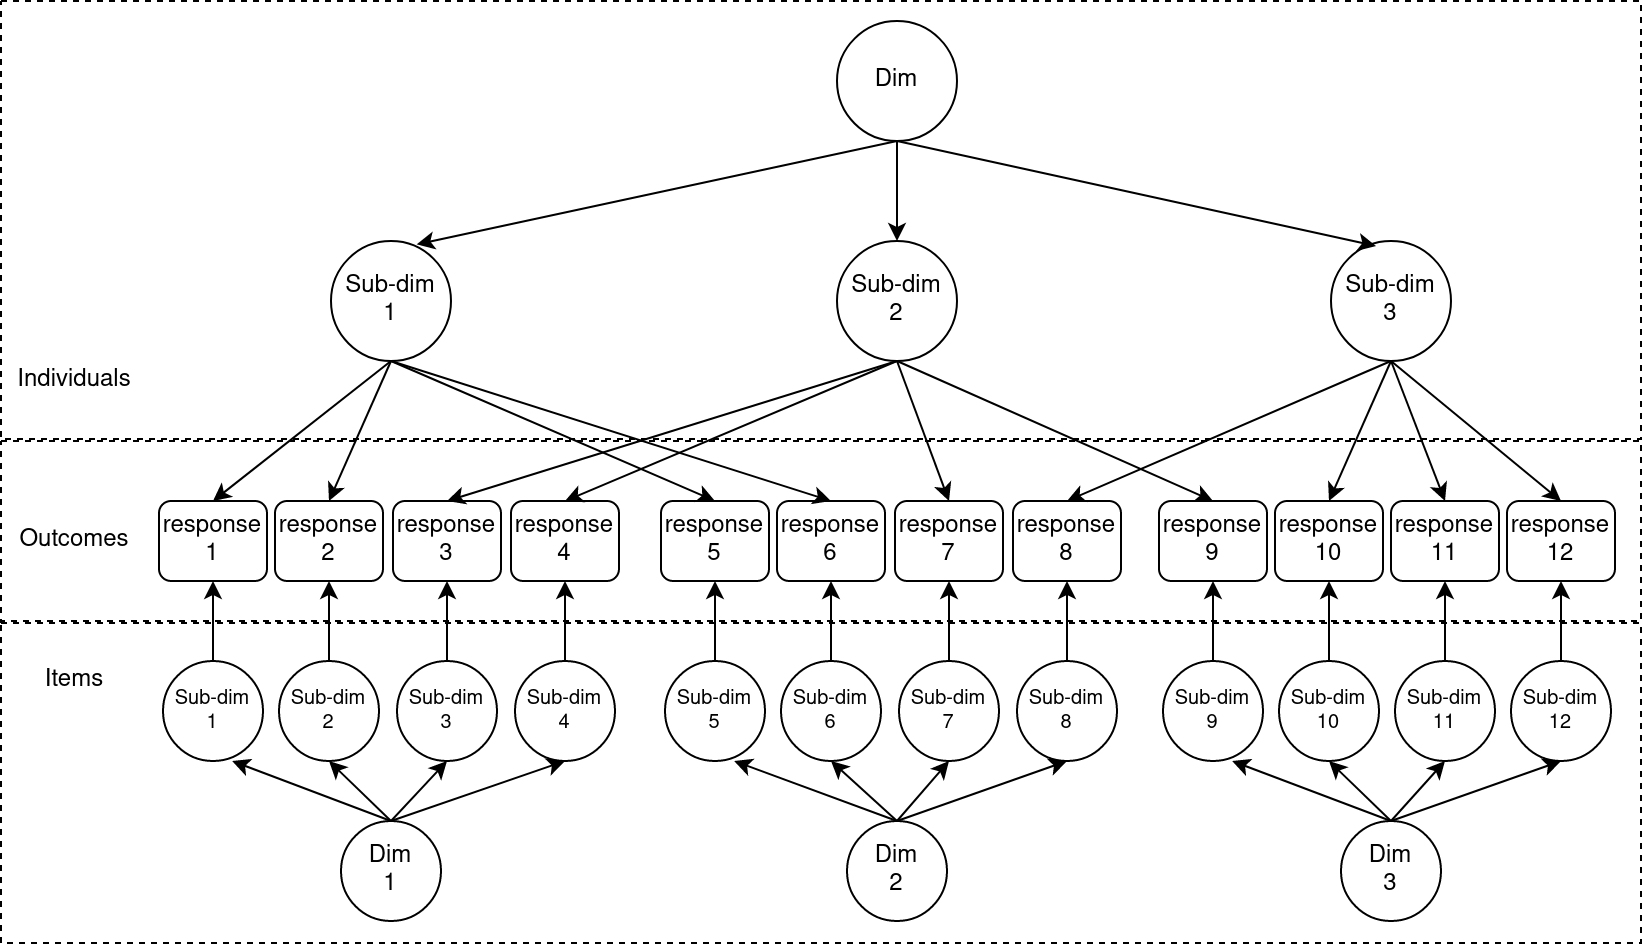
\includegraphics[width=0.95\textwidth]{instrument_design}
			\caption{Path diagram of the dimensional structure for a hierarchical cross-classified IRT model.}
			\label{fig:design}
		\end{figure}
		%
	\end{frame}
	%
	%---------------------------
	\begin{frame}
		%
		\frametitle{Motivating example (cont.)}
		%
		\begin{itemize}
			%
			\item Empty level-1 covariates matrix $\mathbf{X}_{j}$ ($P=0$)
			%
			\item $M=2$ levels at the items block, with $K_{2}=12$ and $K_{3}=3$, i.e. $\pmb{\eta}^{(2)} = [ \eta_{1}^{(2)}, \dots, \eta_{12}^{(2)} ]^{T}$ and $\pmb{\eta}^{(3)} = [ \eta_{1}^{(3)}, \eta_{2}^{(3)}, \eta_{3}^{(3)} ]^{T}$
			%
			\item $L=2$ levels in the individuals block, with $D_{2}=3$ and $D_{3}=1$, i.e. $\pmb{\theta}^{(2)} = [ \theta_{1}^{(2)}, \theta_{2}^{(2)}, \theta_{3}^{(2)} ]^{T}$ and $\pmb{\theta}^{(3)} = \theta_{1}^{(3)}$.
			%
			\item Specific regression relationship among latents $\pmb{\Psi}$, i.e.
			$ \pmb{\alpha}^{(3)} = [ \alpha_{11}^{(3)}, \dots, \alpha_{15}^{(3)}, \alpha_{21}^{(3)}, \dots, \alpha_{25}^{(3)}, \alpha_{31}^{(3)}, \dots, \alpha_{35}^{(3)} ]^{T} $ and  $ \pmb{\lambda}^{(3)} = [ \lambda_{1}^{(3)}, \lambda_{2}^{(3)}, \lambda_{3}^{(3)} ]^{T}$ 
			%
			\item Empty structural covariates $\mathbf{W}$.
			%
		\end{itemize}
		%
	\end{frame}
	%
	%
	%%%%%%%%%%%%%%%%%%%%%%%%%%%%%%%%%%%%%%%%%%%%%%%%%%%%%%%%%%%%%%%%%
	\section{3. Bayesian estimation}
	%%%%%%%%%%%%%%%%%%%%%%%%%%%%%%%%%%%%%%%%%%%%%%%%%%%%%%%%%%%%%%%%%
	%
	\begin{frame}
		%
		\LARGE{\textbf{3. Bayesian Estimation}}
		%
	\end{frame}
	%
	%---------------------------
	\begin{frame}
		%
		\frametitle{Bayesian GLLAMM for dichotomous outcomes}
		%
		\begin{enumerate}
			%
			\item \textbf{Posterior distribution.}
			Given that $\mathbf{Y}$ is the observed data and $\pmb{\Omega} = \{ \pmb{\beta}, \pmb{\Lambda}, \pmb{\Theta}, \pmb{\Psi}, \pmb{\Gamma} \}$ the parameters:
			%
			\begin{equation} \label{eq:posterior1}
				\begin{split}
					P(\pmb{\Omega} \; | \; \mathbf{Y}) &= \frac{ P( \mathbf{Y} \; | \; \pmb{\Omega} ) \; P( \pmb{\Omega} ) }{ \int P( \mathbf{Y} \; | \; \pmb{\Omega} ) \; P( \pmb{\Omega} ) \; d\pmb{\Omega} }
				\end{split}
			\end{equation}
			%
			\item \textbf{Prior distributions} $P(\pmb{\Omega})$.
			Similar to \citet{Patz_et_al_1999}, we use an independent distributional structure for the joint priors:
			%
			\begin{equation}
				\begin{split}
					P( \pmb{\Omega} ) =& P( \pmb{\beta} ) \; P( \pmb{\Lambda} ) \; P( \pmb{\Theta} ) \; P( \pmb{\Psi} ) \; P( \pmb{\Gamma}) \\
					%
					=& P( \pmb{\beta} ) \; \left[ P( \pmb{\alpha} ) \; P( \pmb{\lambda} ) \right] \; \left[ P( \pmb{\eta} ) \; P( \pmb{\theta} ) \right] \\
					%
					& \left[ P( \pmb{\Psi}_{\eta} ) \; P( \pmb{\Psi}_{\theta} ) \right] \; \left[ P( \pmb{\Gamma}_{\eta} ) \; P( \pmb{\Gamma}_{\theta} ) \right]
				\end{split}
			\end{equation}
			%
		\end{enumerate}
		%
	\end{frame}
	%
	%---------------------------
	\begin{frame}
		%
		\frametitle{Bayesian GLLAMM for dichotomous outcomes (cont.)}
		%
		\begin{enumerate}
			\setcounter{enumi}{2}
			%
			\item \textbf{Likelihood} $P( \mathbf{Y} \; | \; \pmb{\Omega} )$.
			Following \citet{Rabe_et_al_2004a}, the likelihood function is build in a recursive way. 
		\end{enumerate}
		%
		\vspace{0.3cm} \begin{equation} \label{eq:lik1}
			f \left( \mathbf{y}=\mathbf{1} \; | \; \mathbf{X}, \mathbf{W}, \pmb{\Omega} \right) = \prod_{j=1}^{J} \prod_{d=1}^{D} \prod_{k=1}^{K} f \left( y_{jkd}=1 \; | \; \mathbf{X}, \mathbf{W}, \pmb{\Omega} \right)
		\end{equation}
		%
		\begin{equation} \label{eq:lik2}
			f^{(l)}_{(m)} \left( \mathbf{y}=\mathbf{1} \; | \; \mathbf{X}, \mathbf{W}, \pmb{\Omega} \right) = \int \left[ \prod f^{(l-1)}_{(m-1)} \left( \mathbf{y}=\mathbf{1} \; | \; \mathbf{X}, \mathbf{W}, \pmb{\Omega} \right) \right] \; P( \pmb{\Theta}^{(l)}_{(m)} ) \; d\pmb{\Theta}^{(l)}_{(m)}
		\end{equation}
		%
		%
		\begin{equation} \label{eq:lik3}
			\mathcal{L}(\mathbf{X}, \mathbf{W}, \pmb{\Omega}) = \prod_{m=2}^{M+1} \prod_{l=2}^{L+1} f^{(l)}_{(m)} \left( \mathbf{y}=\mathbf{1} \; | \; \mathbf{X}, \mathbf{W}, \pmb{\Omega} \right)
		\end{equation}
		%
		%
		\begin{equation} \label{eq:loglik}
			\ell(\mathbf{X}, \mathbf{W}, \pmb{\Omega}) = \log \mathcal{L}(\mathbf{X}, \mathbf{W}, \pmb{\Omega})
		\end{equation}
		%
	\end{frame}
	%
	%---------------------------
	\begin{frame}
		%
		\frametitle{Computational implementation}
		%
		\begin{enumerate}
			%\setcounter{enumi}{2}
			%
			\item Hamiltonian Monte Carlo (HMC) and \texttt{Stan} \cite{Stan2020}.
			%
			\item \textbf{No burn-in and thinning}. Warm-up phase to ``tune-up" the number of steps (\texttt{leapfrogs}), and the \texttt{step size} \cite{Stan2020}.
			%
			\item We use $3,000$ \textbf{effective iterations}: $3$ chains of $2,000$ iterations each, where $1,000$ are spend on warm-up.
			%
			\item \textbf{Initial starts} sampled from the priors defined in the model.
			%
			\item Prior distributions selected based on \textbf{prior predictive simulations}.
			%
			\item We test the \textbf{centered (CP)} and \textbf{non-centered parametrizations (NCP)}.
			%
		\end{enumerate}
		%
	\end{frame}
	%
	%
	%
	%%%%%%%%%%%%%%%%%%%%%%%%%%%%%%%%%%%%%%%%%%%%%%%%%%%%%%%%%%%%%%%%%
	\section{4. Simulation study}
	%%%%%%%%%%%%%%%%%%%%%%%%%%%%%%%%%%%%%%%%%%%%%%%%%%%%%%%%%%%%%%%%%
	%
	\begin{frame}
		%
		\LARGE{\textbf{4. Simulation studies}}
		%
	\end{frame}
	%
	%---------------------------
	\begin{frame}
		%
		\frametitle{Objectives}
		%
		\begin{enumerate}
			%
			\item \textbf{Performance.} In terms of achieving ergodicity, under the CP and NCP, 
			%
			\item \textbf{Recovery capacity.} Capacity to recover the parameters of interest, especially the structural regression parameters.
			%
			\item \textbf{Retrodictive accuracy.} Capacity to retrodict the data of interest, according to a set of aggregating dimensions.
			%
		\end{enumerate} 
		%
	\end{frame}
	%
	%---------------------------
	\begin{frame}
		%
		\frametitle{Results \\
			(Performance)}
		%
		\begin{enumerate}
			%
			\item the non-centered parametrization (NCP) largely
			improved the performance of the MCMC chains, towards achieving ergodicity.\\
			%
			\vspace{0.3cm} This is true across models, simulated sample sizes, and simulated replicas.
			%
			\item No large difference in performance was observed in either the sub-dimensions’ correlation or loading parameters.\\
			%
			\vspace{0.3cm} However, no evidence supported the idea the parameters suffered from a further lack of identification.
			%
		\end{enumerate} 
		%
	\end{frame}
	%
	%---------------------------
	\begin{frame}
		%
		\frametitle{Results \\
			(Performance, cont.)}
		%
		\begin{figure}[H]
			\centering
			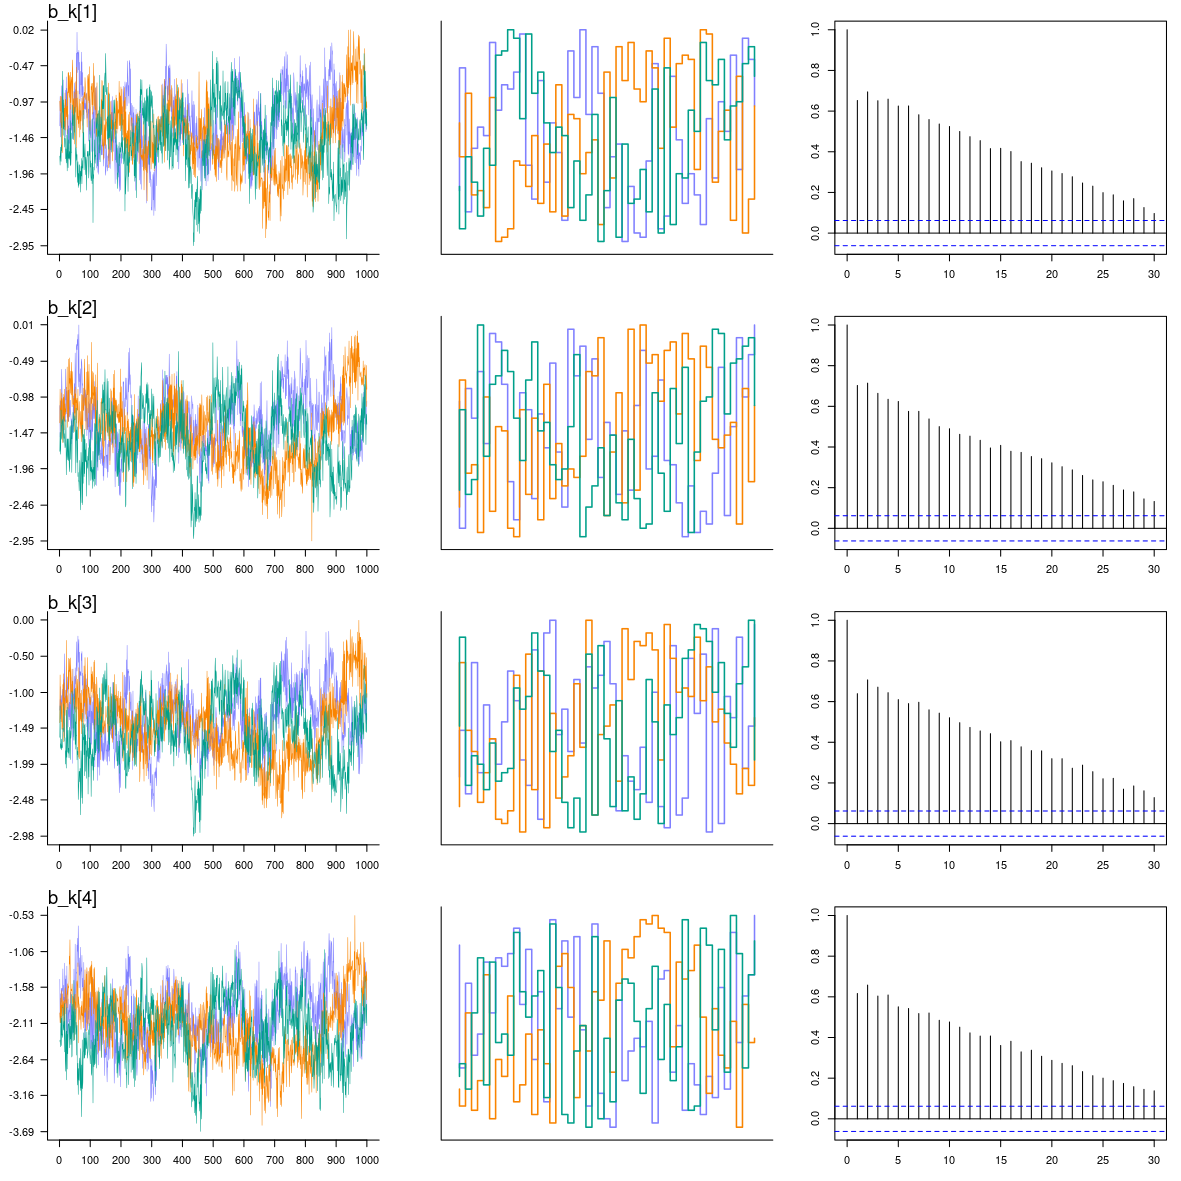
\includegraphics[width=0.60\linewidth]{FOLV_CE_J100_Ndata1_bk1}
			\caption{First-order latent variable model (FOLV). Sample size $100$, replica number $1$. Centered parametrization. Item Difficulties.}
			\label{fig:FOLV_CE_chains3}
		\end{figure} 
		%
	\end{frame}
	%
	%---------------------------
	\begin{frame}
		%
		\frametitle{Results \\
			(Performance, cont.)}
		%
		\begin{figure}[H]
			\centering
			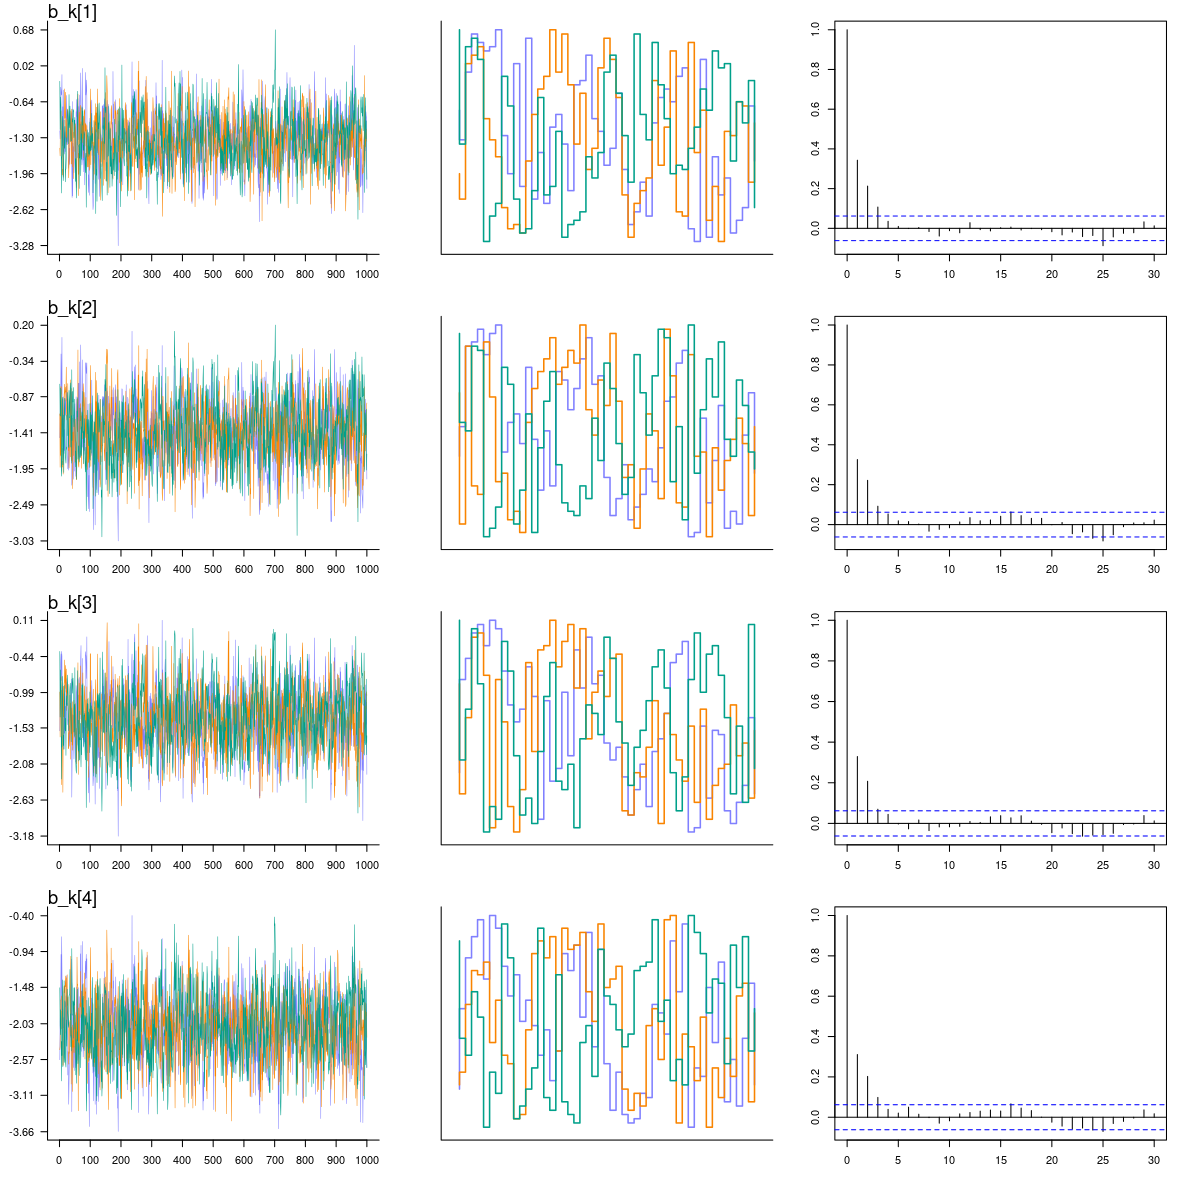
\includegraphics[width=0.60\linewidth]{FOLV_NC_J100_Ndata1_bk1}
			\caption{First-order latent variable model (FOLV). Sample size $100$, replica number $1$. Non-centered parametrization. Item Difficulties.}
			\label{fig:FOLV_NC_chains3}
		\end{figure} 
		%
	\end{frame}
	%
	%---------------------------
	\begin{frame}
		%
		\frametitle{Results \\
			(Recovery capacity)}
		%
		\begin{enumerate}
			%
			\item The GLLAMM was able to recover most of the simulated parameters with good precision.
			%
			\item However, the model still had issues estimating the sub-dimensions correlations and loadings.\\
			%
			\vspace{0.3cm} Under the Confirmatory Factor Analysis theory (CFA), a SOLV model is only justified, if the lower-level correlations are high enough, usually above 0.8.
			%
			%
			\item It is surprising that CP and NCP achieved similar levels of recovery capacity.
			%
		\end{enumerate} 
		%
	\end{frame}
	%
	%---------------------------
	\begin{frame}
		%
		\frametitle{Results \\
			(Recovery capacity, cont.)}
		%
		\begin{figure}[H]
			\centering
			%\begin{subfigure}
			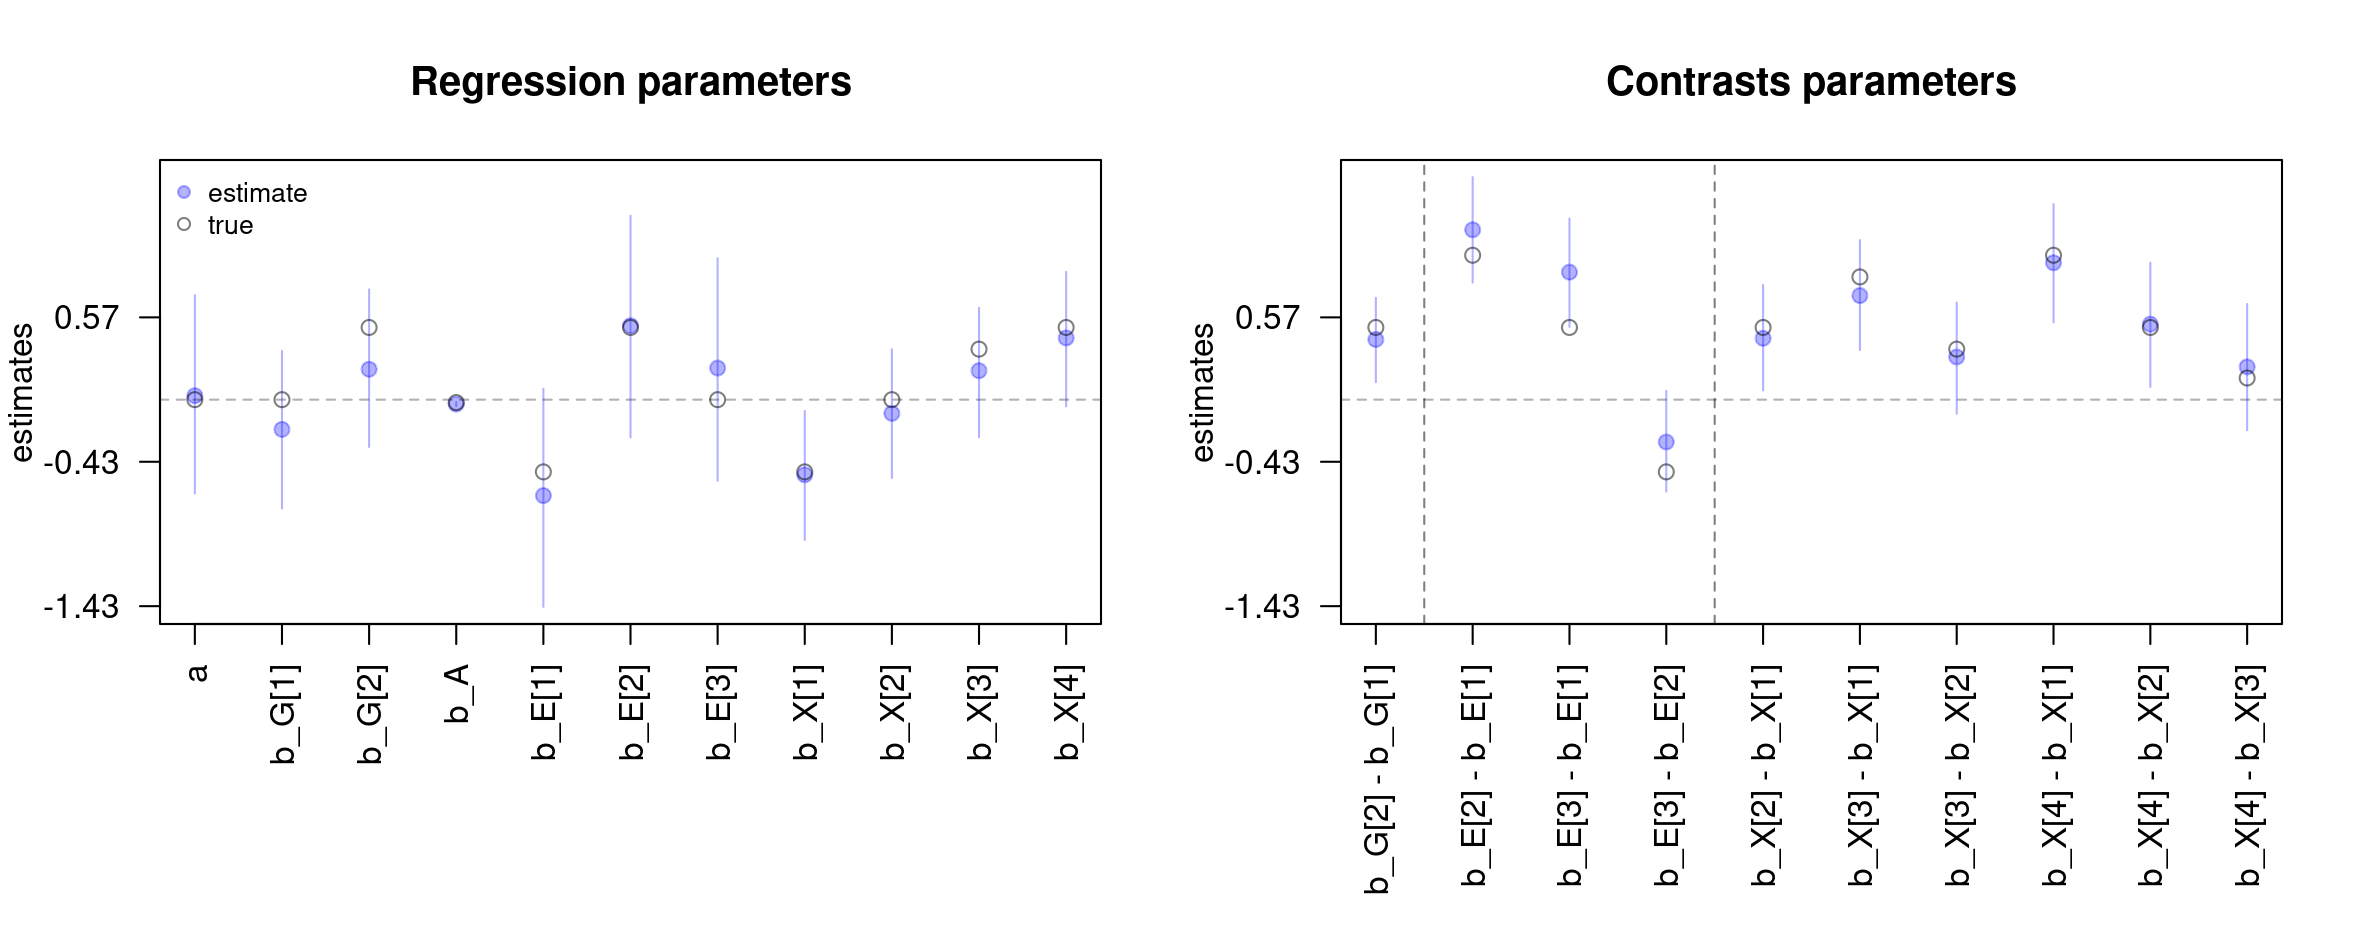
\includegraphics[width=0.65\linewidth]{FOLV_NC_J100_Ndata1_regression}
			%\end{subfigure}
			%
			%\begin{subfigure}
			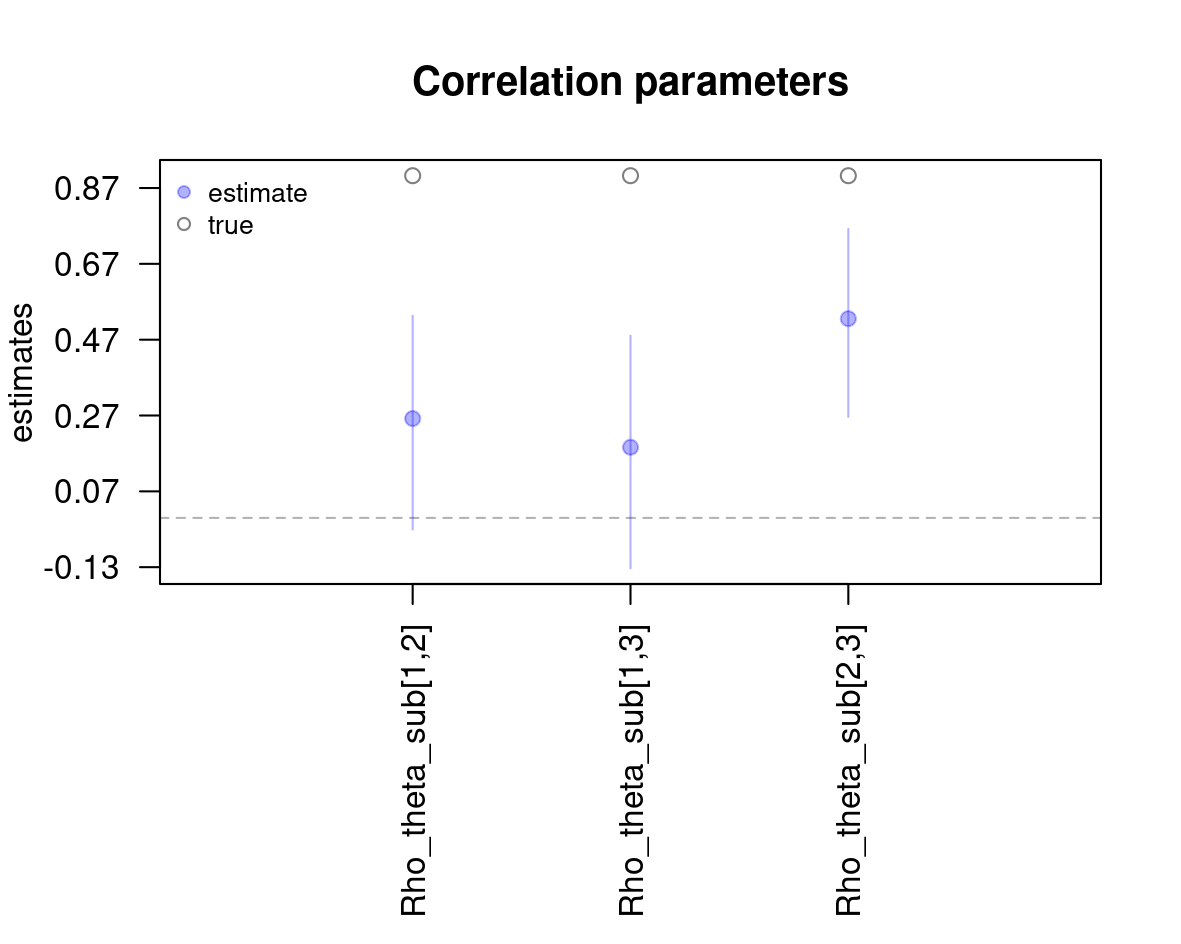
\includegraphics[width=0.35\linewidth]{FOLV_NC_J100_Ndata1_corr}
			%\end{subfigure}
			\caption{First-order latent variable model (FOLV). Non-centered parametrization. Sample size $100$, replica $1$. Regression, contrast, and correlation parameters.}
			\label{fig:FOLV_NC_recovery1}
		\end{figure} 
		%
	\end{frame}
	%
	%---------------------------
	\begin{frame}
		%
		\frametitle{Results \\
			(Retrodictive accuracy)}
		%
		\begin{enumerate}
			%
			\item the models managed to capture the traits of the data, while avoiding its exact replication.\\
			%
			\vspace{0.3cm} These result were consistent across models, simulated sample sizes and replicas.
			%
		\end{enumerate} 
		%
	\end{frame}
	%
	%---------------------------
	\begin{frame}
		%
		\frametitle{Results \\
			(Retrodictive accuracy, cont.)}
		%
		\begin{figure}[H]
			\centering
			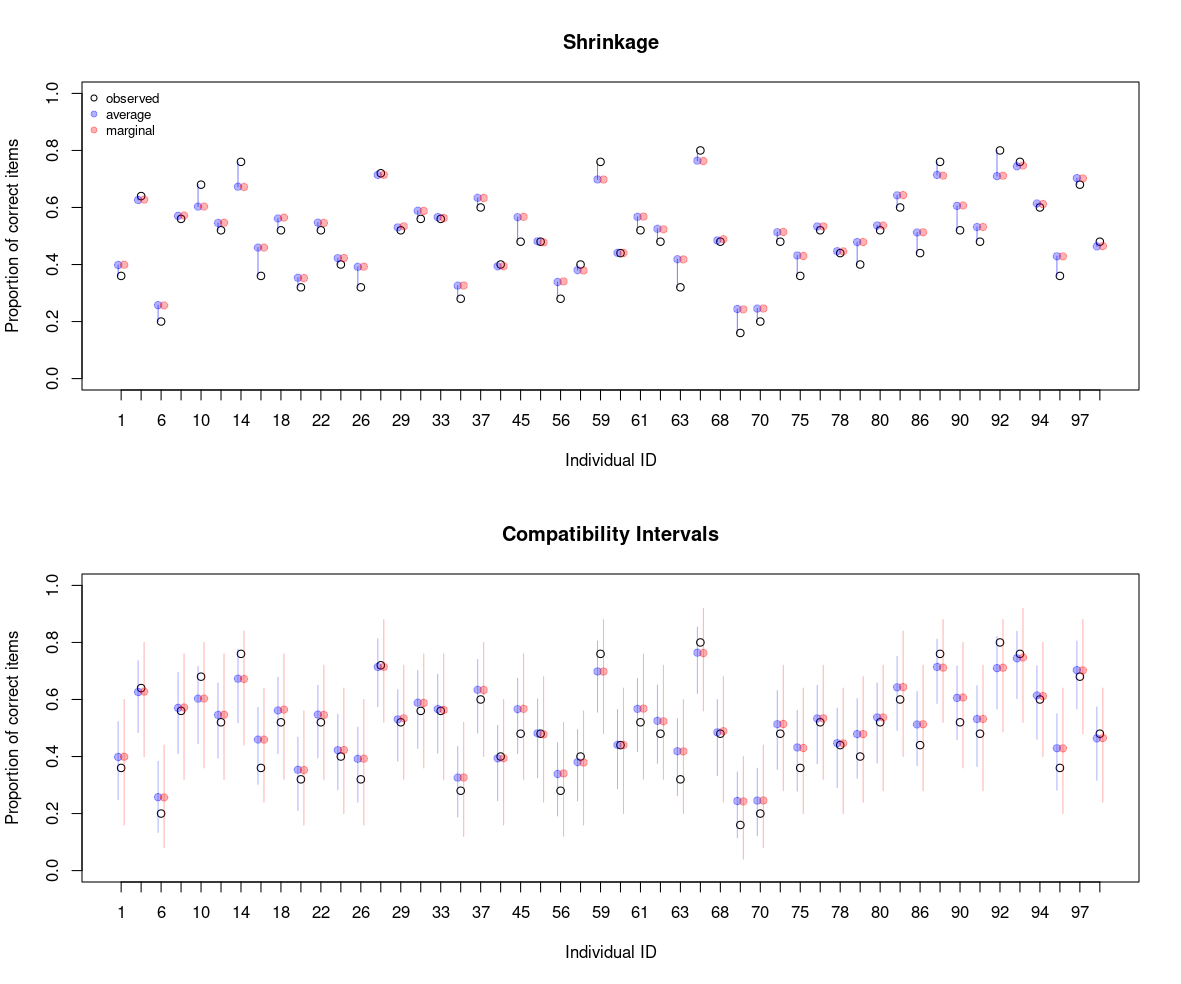
\includegraphics[width=0.68\linewidth]{FOLV_NC_J100_Ndata4_HitRate_ind}
			\caption{First-order latent variable model (FOLV). Sample size $100$, replica number $4$. Non-centered parametrization. Individual predictive plot.}
			\label{fig:FOLV_NC_hitrate_ind}
		\end{figure} 
		%
	\end{frame}
	%
	%
	%%%%%%%%%%%%%%%%%%%%%%%%%%%%%%%%%%%%%%%%%%%%%%%%%%%%%%%%%%%%%%%%%
	\section{5. Application}
	%%%%%%%%%%%%%%%%%%%%%%%%%%%%%%%%%%%%%%%%%%%%%%%%%%%%%%%%%%%%%%%%%
	%
	\begin{frame}
		%
		\LARGE{\textbf{5. Application}}
		%
	\end{frame}
	%
	%---------------------------
	\begin{frame}
		%
		\frametitle{Objectives}
		%
		\begin{enumerate}
			%
			\item \textbf{Evaluate the performance of the parametrizations.} Ergodicity of CP vs NCP.
			%
			\item \textbf{Evaluate the retrodictive accuracy.}
			%
			\item \textbf{Assess the psychometric properties.} Special interest in determine how difficult the items were.
			%
			\item \textbf{Test research hypothesis.} About the explanatory power a set of covariates had on the latent dimensions, and their implications for the educational authority.
			%
		\end{enumerate}
		%
	\end{frame}
	%
	%---------------------------
	\begin{frame}
		%
		\frametitle{Instrument and data}
		%
		\begin{enumerate}
			%
			\item \textbf{Instrument.} Reading comprehension sub-test composed of $25$ binary scored items, from the Peruvian public teaching career national assessment.
			%
			\item \textbf{Access.} Legal requirement of open information to
			the Ministry of Education of Peru (MINEDU).
			%
			\item \textbf{Sample scheme.} Simple random sample of $2,000$ (from approx. $195,0000$).
			%
		\end{enumerate} 
		%
	\end{frame}
	%
	%---------------------------
	\begin{frame}
		%
		\frametitle{Results \\
			(Performance)}
		%
		\begin{enumerate}
			%
			\item the non-centered parametrization (NCP) largely
			improved the performance of the MCMC chains, towards achieving ergodicity.
			%
			\item No large difference in performance was observed in either the sub-dimensions’ correlation or loading parameters.\\
			%
			\vspace{0.3cm} results are similar to simulation study, albeit in some cases more extreme.
			%
		\end{enumerate} 
		%
	\end{frame}
	%
	%---------------------------
	\begin{frame}
		%
		\frametitle{Results \\
			(Performance, cont.)}
		%
		\begin{figure}[H]
			\centering
			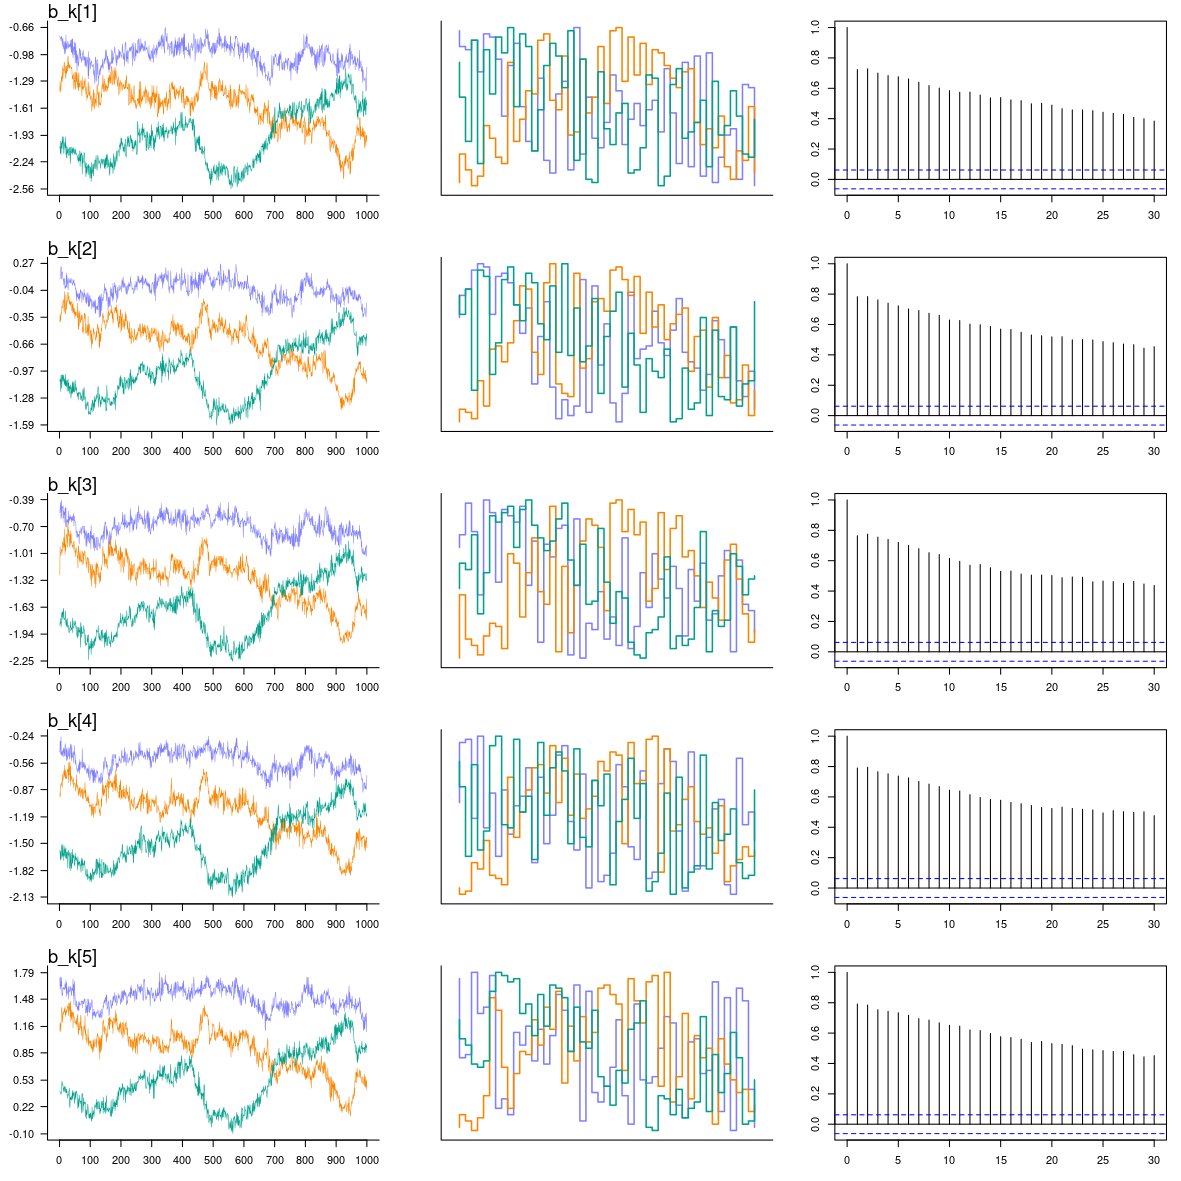
\includegraphics[width=0.60\linewidth]{FOLV_CE_bk_1_5}
			\caption{Application’s first-order latent variable model (FOLV). Centered parametrization. Item difficulties.}
			\label{fig:FOLV_CE_chains1}
		\end{figure} 
		%
	\end{frame}
	%
	%---------------------------
	\begin{frame}
		%
		\frametitle{Results \\
			(Performance, cont.)}
		%
		\begin{figure}[H]
			\centering
			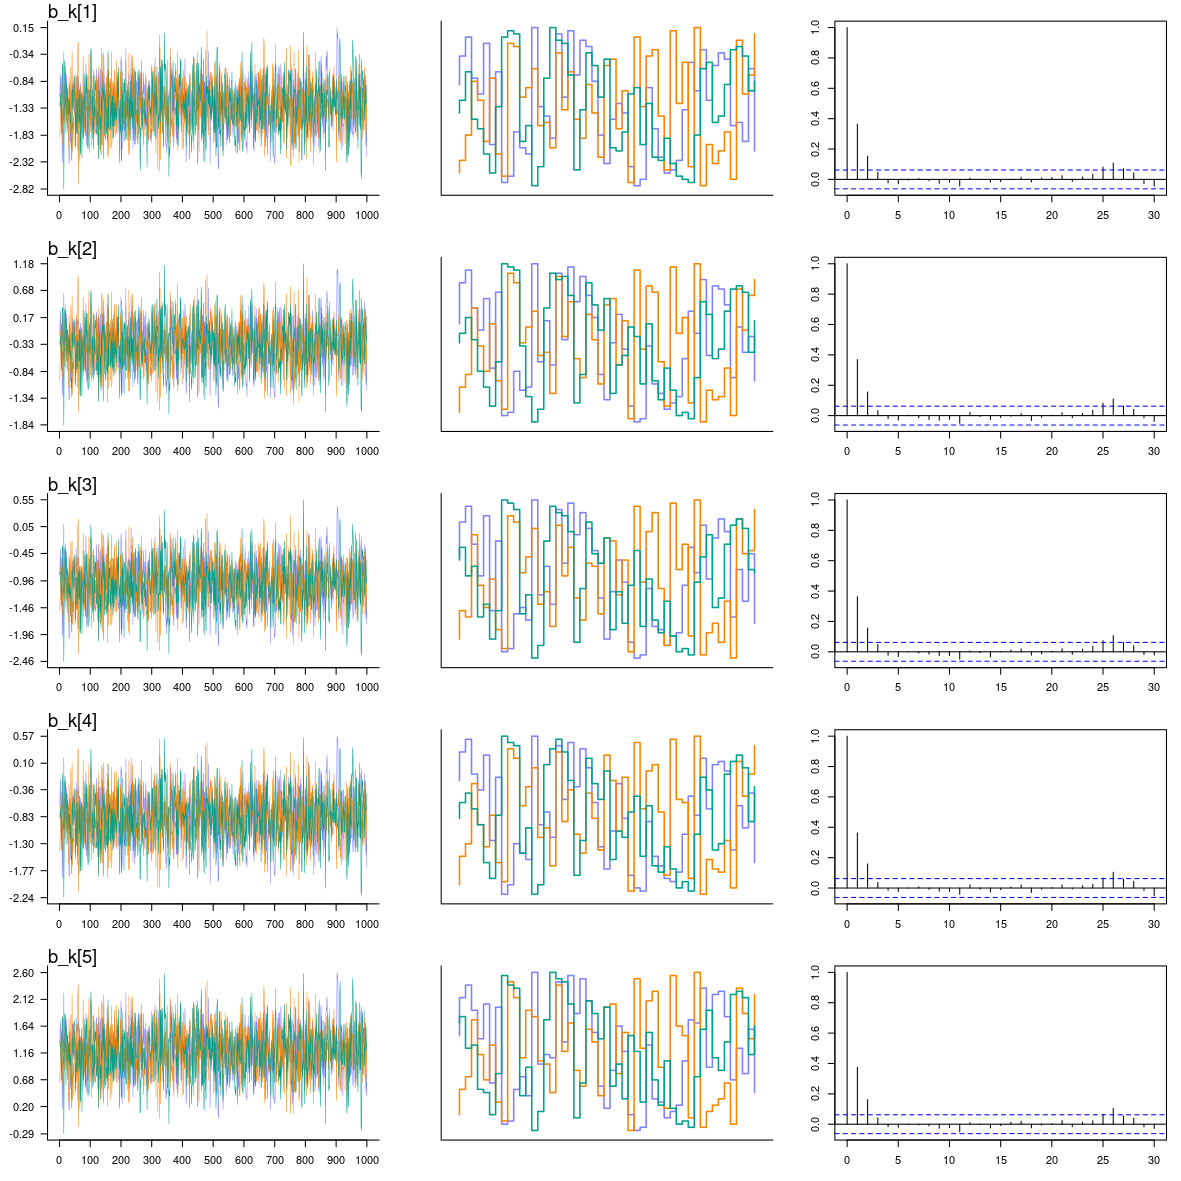
\includegraphics[width=0.60\linewidth]{FOLV_NC_bk_1_5}
			\caption{Application’s first-order latent variable model (FOLV). Non-centered parametrization. Item difficulties.}
			\label{fig:FOLV_NC_chains1}
		\end{figure} 
		%
	\end{frame}
	%
	%---------------------------
	\begin{frame}
		%
		\frametitle{Results \\
			(Retrodictive accuracy)}
		%
		\begin{enumerate}
			%
			\item the models managed to capture the traits of the data, while avoiding its exact replication.\\
			%
			\vspace{0.3cm} Similar to simulation study.
			%
		\end{enumerate} 
		%
	\end{frame}
	%
	%---------------------------
	\begin{frame}
		%
		\frametitle{Results \\
			(Retrodictive accuracy, cont.)}
		%
		\begin{figure}[H]
			\centering
			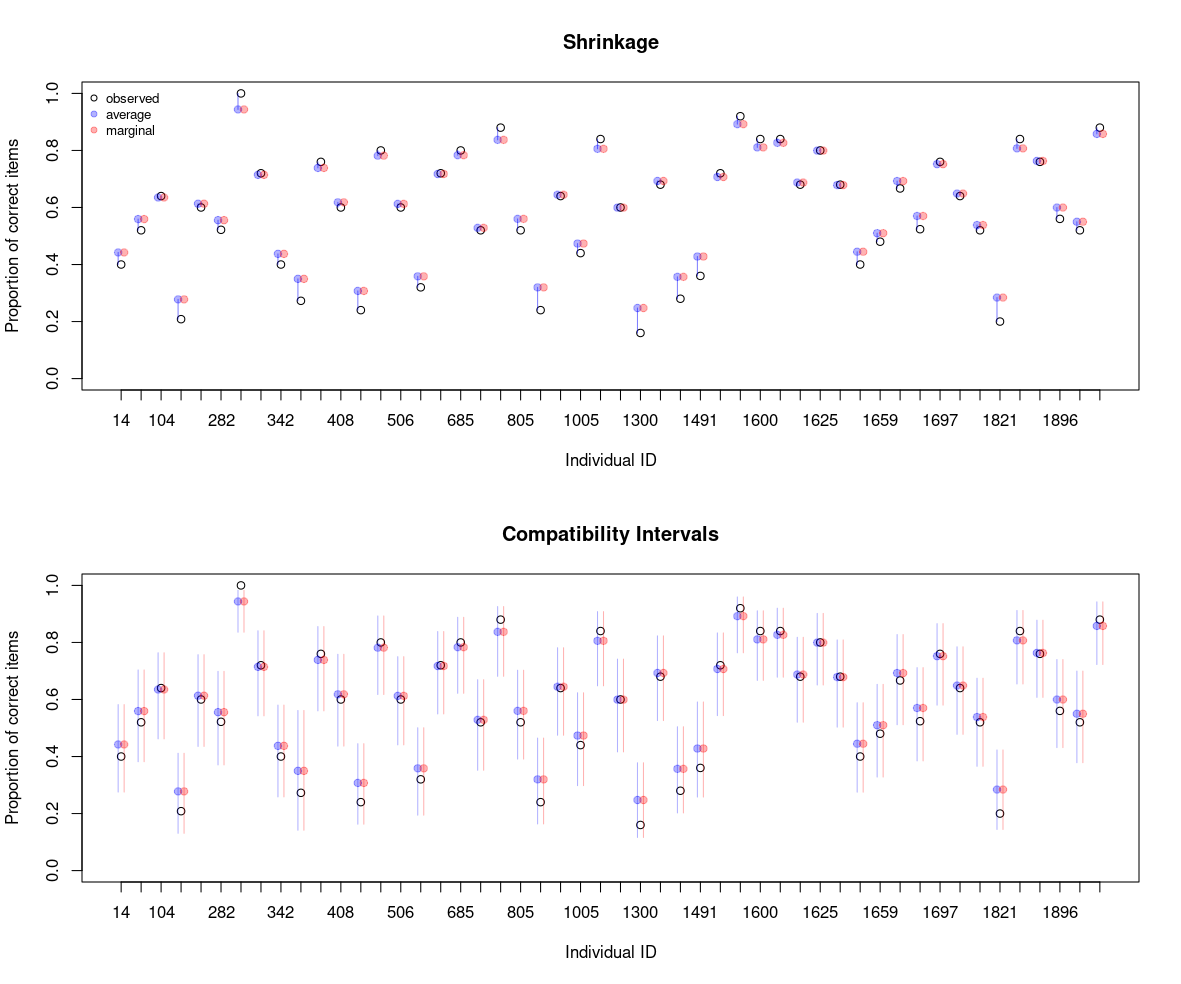
\includegraphics[width=0.70\linewidth]{FOLV_NC_HitRate_ind}
			\caption{First-order latent variable model (FOLV). Non-centered parametrization. Individual predictive plot.}
			\label{fig:FOLV_pred_app}
		\end{figure} 
		%
	\end{frame}
	%
	%---------------------------
	\begin{frame}
		%
		\frametitle{Results \\
			(Psychometric properties)}
		%
		\begin{enumerate}
			%
			\item the items were scattered throughout a significant portion of the abilities range. 
			%
			\item Specific benefit of the implementation allowed us to assess
			how difficult the texts were.
			%
			\item (a word of advice) A more sound psychometric analysis requires access to the items and texts description, but it was not possible due to legal restrictions.
			%
		\end{enumerate} 
		%
	\end{frame}
	%
	%---------------------------
	\begin{frame}
		%
		\frametitle{Results \\
			(Psychometric properties, cont.)}
		\begin{figure}[H]
			\centering
			%\begin{subfigure}
			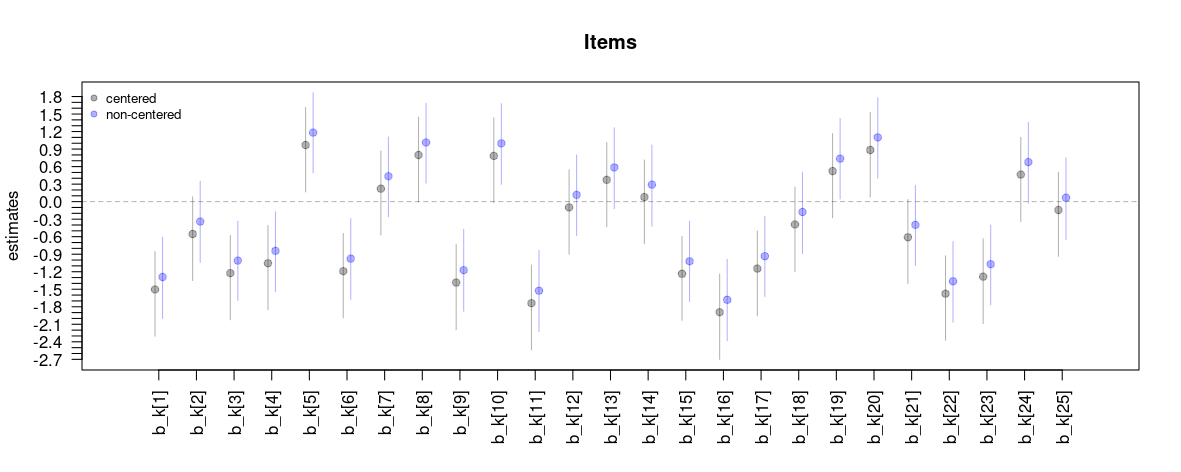
\includegraphics[width=0.70\linewidth]{FOLV_recovery_items}
			%\end{subfigure}
			%
			%\begin{subfigure}
			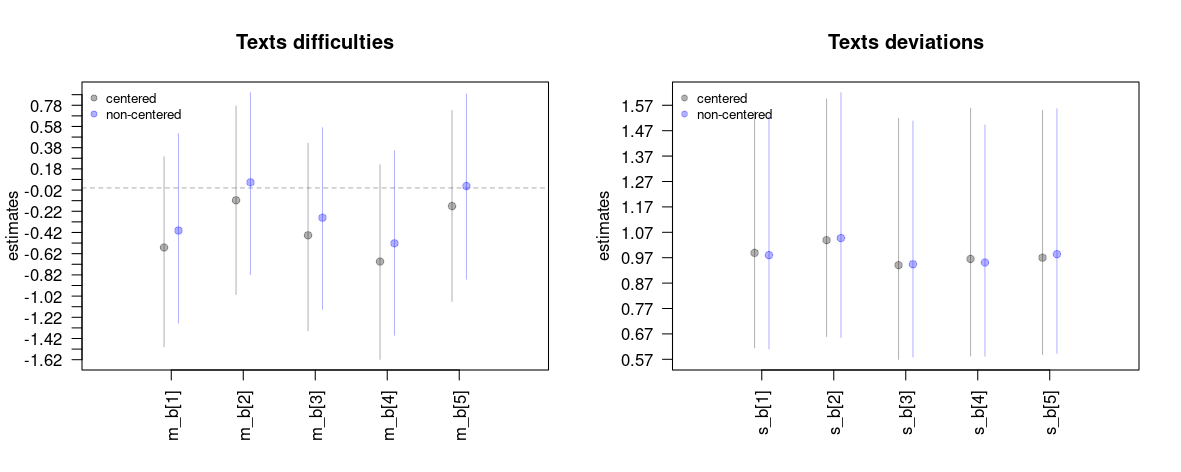
\includegraphics[width=0.69\linewidth]{FOLV_recovery_texts}
			%\end{subfigure}
			%
			\caption{First-order latent variable model (FOLV). Centered and non-centered parametrization. Items, texts difficulties, and texts deviations.}
			\label{fig:FOLV_CE.NC_recovery}
		\end{figure}
		%
	\end{frame}
	%
	%---------------------------
	\begin{frame}
		%
		\frametitle{Results \\
			(Hypothesis testing)}
		%
		\begin{figure}[H]
			\centering
			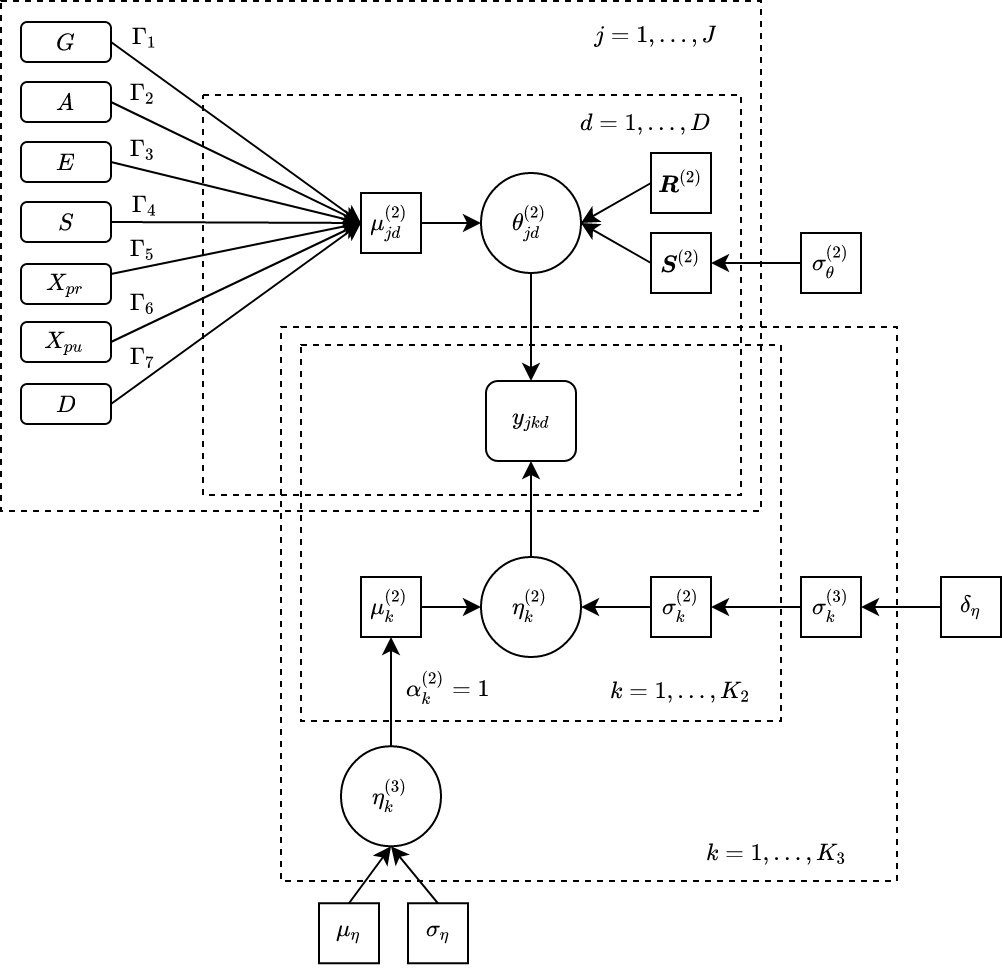
\includegraphics[width=0.75\linewidth]{app_FOLV_dag}
			\caption{Directed Acyclig Graph (DAG). Application’s first-order latent variable model (FOLV).}
			\label{fig:FOLV_app}
		\end{figure}
		%
	\end{frame}
	%
	%---------------------------
	\begin{frame}
		%
		\frametitle{Results \\
			(Hypothesis testing, cont.)}
		%
		\begin{enumerate}
			%
			\item Age (style of teaching proxy) explains negatively reading comprehension $-0.036[-0.04, -0.03]$.
			%
			\item Disability also explained the the reading comprehension sub-dimensions, although the results were mildly unexpected. 
			%
			\item the statistical evidence seem to support the lower quality of training on pedagogical institutes.
			%
			\item Experience improved the reading comprehension abilities. Private experience effects were larger than the public. We observe also diminishing returns on abilities, as the years of experience increases.
			%
			\item Instructing students from secondary education improves reading comprehension.
			%
		\end{enumerate} 
		%
	\end{frame}
	%
	%---------------------------
	\begin{frame}
		%
		\frametitle{Results \\
			(Hypothesis testing, cont.)}
		\begin{figure}[H]
			\centering
			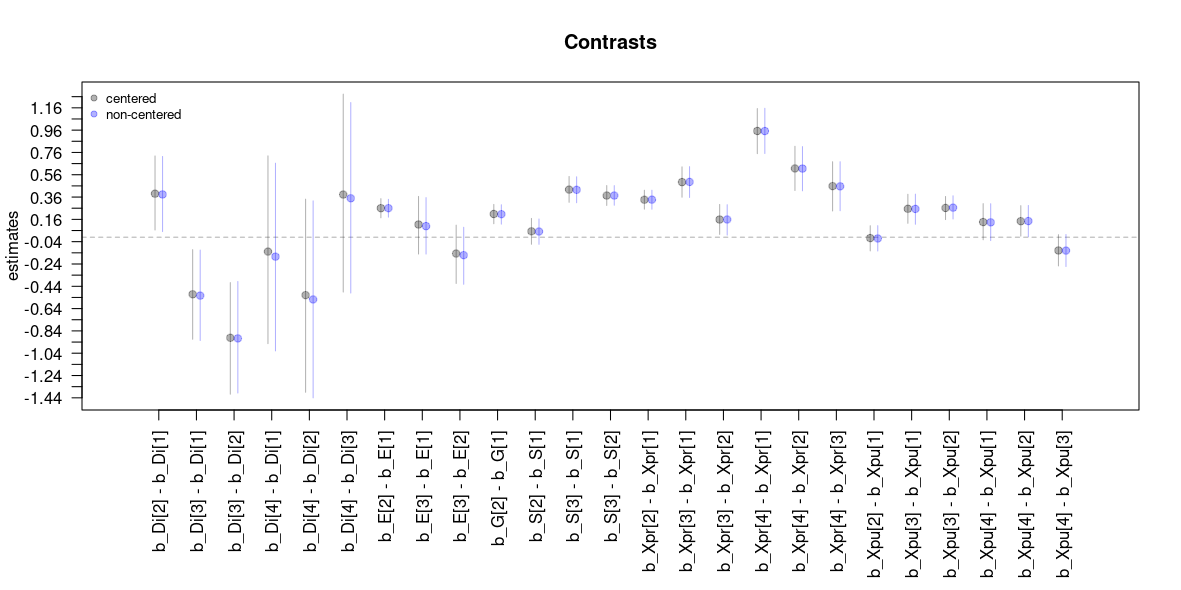
\includegraphics[width=1\linewidth]{FOLV_recovery_contrast}
			\caption{Application’s first-order latent variable model (FOLV). CP and NCP comparison plot. Contrasts.}
			\label{fig:contrast_both}
		\end{figure}
		%
	\end{frame}
	%
	%
	%%%%%%%%%%%%%%%%%%%%%%%%%%%%%%%%%%%%%%%%%%%%%%%%%%%%%%%%%%%%%%%%%
	\section{6. Conclusions}
	%%%%%%%%%%%%%%%%%%%%%%%%%%%%%%%%%%%%%%%%%%%%%%%%%%%%%%%%%%%%%%%%%
	%
	\begin{frame}
		%
		\LARGE{\textbf{6. Conclusions and further development}}
		%
	\end{frame}
	%
	%---------------------------
	\begin{frame}
		%
		\frametitle{Conclusions}
		%
		\begin{enumerate}
			\item The NCP \textbf{largely improved the performance} of the MCMC chains. True in simulations, and under the real application, albeit with some caveats.
			%
			\item The proposed model \textbf{recovered most of the simulated parameters} with good precision. The model still had issues with the sub-dimensions correlations and loadings.
			%
			\item The models managed to \textbf{capture the traits of the data}, while \textbf{avoiding its exact replication}. Consistent in simulations, and under the real application.
			%
			\item The NCP was \textbf{slightly faster} than the CP, although the magnitudes of the differences in running time were not large.
			%
			\item On the real application, the model \textbf{provided the (extra) benefit} to asses the psychometric properties of texts.
			%
			\item Finally, the model produced \textbf{interesting statistical results}, supported by the statistical application and the DAG guiding our interpretation and causal assumptions.
			%
		\end{enumerate}
		%
	\end{frame}
	%
	%---------------------------
	\begin{frame}
		%
		\frametitle{Further investigation}
		%
		\begin{enumerate}
			\item Why the benefits of the NCP did not fully extend to correlations and loadings?.
			%
			\item Why the CP (no ergodicity) managed recover the parameters as good as the NCP.
			%
			\item Similar to HMC, test results for Variational Inference methods (VI)
			%
			\item The statistical evidence remains valid with a better sample scheme?
			%
			\item Test the model also with response explanatory variables, e.g. response time, number of alternatives, etc.
			%
			\item Test the model for measurement invariance.
			%
		\end{enumerate}
		%
	\end{frame}
	%
	%---------------------------
	\begin{frame}
		%
		\LARGE{\textbf{Thank you!}}
		% 
	\end{frame}
	%
	%
	%%%%%%%%%%%%%%%%%%%%%%%%%%%%%%%%%%%%%%%%%%%%%%%%%%%%%%%%%%%%%%%%%
	\section*{Appendix}
	%%%%%%%%%%%%%%%%%%%%%%%%%%%%%%%%%%%%%%%%%%%%%%%%%%%%%%%%%%%%%%%%%
	%
	\begin{frame}
		%
		\LARGE{\textbf{Appendix}}
		%
	\end{frame}
	%
	%---------------------------
	\begin{frame}
		%
		\frametitle{Improving MCMC chain performance}
		%
		Four solutions are offered to solve the previous pathologies:
		%
		\begin{itemize}
			\item Changing the settings of the MCMC method
			%
			\begin{enumerate}
				\item increasing the number of iterations per chain, with large burn-in and thinning processes
				%
				\item designing model-specific MCMC algorithms.
				%
			\end{enumerate}
			%
			\item Readjusting the Bayesian model
			%
			\begin{enumerate}
				\setcounter{enumi}{2}
				\item re-write the model in an alternative parametrization (\textbf{simple changes})
				%
				\item encode prior information through the prior distributions
				%
			\end{enumerate}
			%
		\end{itemize}
		%
	\end{frame}
	%
	%---------------------------
	\begin{frame}
		%
		\frametitle{Cluster effects}
		%
		Individual clustering involves the addition of more random effects to the linear predictor defined in equation (\ref{eq:linear_predictor2}):
		%
		\begin{equation} \label{eq:linear_predictor4}
			\begin{split}
				v_{jkdc} &= v_{jkd} + \sum_{c=1}^{C} \delta_{c}  \\
				%
				&= v_{jkd} + \pmb{\delta} \mathbf{Z}_{j}
			\end{split}
		\end{equation}
		%
	\end{frame}
	%
	%---------------------------
	\begin{frame}
		%
		\frametitle{Example (restrictions for IRT)}
		%
		we could set the restriction $\pmb{\alpha}^{(2)} = -\pmb{\lambda}^{(2)}$ where $\pmb{\lambda}^{(2)} > \mathbf{0}$. In that case we get a multidimensional generalization of the linear predictor observed in the archetypical Rasch \cite{Rasch_1980}, or 2PL \cite{Lord_et_al_2008} models, i.e. $ \lambda^{(2)}_{d} (\theta^{(2)}_{jd} - \eta^{(2)}_{k} )$ \\
		%
		\vspace{0.3cm} In addition, $\pmb{\alpha}^{(3)} = [ \alpha_{11}^{(3)}, \dots, \alpha_{15}^{(3)}, \alpha_{21}^{(3)}, \dots, \alpha_{25}^{(3)}, , \alpha_{31}^{(3)}, \dots, \alpha_{35}^{(3)} ]^{T}$ $= [1,\dots,1]^{T}$, indicating texts difficulties explain directly the items difficulties at the lower level.
		%
	\end{frame}
	%
	%---------------------------
	\begin{frame}
		%
		\frametitle{Example (restrictions for IRT)}
		Moreover, notice that because in the IRT framework $\pmb{\eta}$ and $\pmb{\theta}$ should be orthogonal to each other by design, we can further decompose equation (\ref{eq:structural_model1}) in the following form:
		%
		\begin{equation} \label{eq:structural_model2}
			\begin{split}
				\pmb{\eta} = \underset{(K \times K)}{\pmb{\Psi}_{\eta}} \underset{(K \times 1)}{\pmb{\eta}} + \underset{(K \times Q)}{\pmb{\Gamma}_{\eta}} \underset{(Q \times 1)}{\mathbf{W}_{\eta}} + \underset{(K \times 1)}{\pmb{\zeta}_{\eta}}
			\end{split}
		\end{equation}
		%
		\begin{equation} \label{eq:structural_model3}
			\begin{split}
				\pmb{\theta} = \underset{(D \times S)}{\pmb{\Psi}_{\theta}} \underset{(D \times 1)}{\pmb{\theta}} + \underset{(D \times Q)}{\pmb{\Gamma}_{\theta}} \underset{(Q \times 1)}{\mathbf{W}_{\theta}} + \underset{(D \times 1)}{\pmb{\zeta}_{\theta}}
			\end{split}
		\end{equation}
		%
	\end{frame}
	%---------------------------
	\begin{frame}
		%
		\frametitle{Model Assumptions}
		Following \citet{Skrondal_et_al_2004a}, the framework has two main assumptions: 
		%
		\begin{enumerate}
			%\setcounter{enumi}{2}
			\item[\textbf{(M1)}] \textbf{Complete latent space.}\citep{Hambleton_et_al_1991b} In the GLLAMM representation, the space is complete if we consider all latent variables $\pmb{\Theta}$ at levels $l > 1$ and $m > 1$.
			%
			\item[\textbf{(M2)}] \textbf{Local Independence.} It assumes independence conditional on all the latent dimensions and covariates, at different hierarchical levels; effectively modeling all the observed dependencies.
			%
		\end{enumerate}
		%
	\end{frame}
	%
	%---------------------------
	\begin{frame}
		%
		\frametitle{Model Assumptions (cont.)}
		\textbf{Local Independence} is defined as follows:
		%
		\begin{equation} \label{eq:independence}
			f \left( \mathbf{y} = \mathbf{1} \; | \; \mathbf{X}, \mathbf{W}, \pmb{\Omega} \right) = \prod_{j=1}^{J} \prod_{d=1}^{D} \prod_{k=1}^{K} f \left( y_{jkd}=1 \; | \; \mathbf{X}, \mathbf{W}, \pmb{\Omega} \right)
		\end{equation}
		%
		\vspace{0.3cm} and comes from:
		%
		\begin{enumerate}
			%
			\item \textbf{Local item independence,}
			%
			\begin{equation}
				f \left( y_{j..}=1 \; | \; \mathbf{X}, \mathbf{W}, \pmb{\Omega} \right) = \prod_{d=1}^{D} \prod_{k=1}^{K} f \left( y_{jkd}=1 \; | \; \mathbf{X}, \mathbf{W}, \pmb{\Omega} \right)
			\end{equation}
			%
			\item \textbf{Local individual independence,}
			%
			\begin{equation}
				f \left( y_{.kd}=1 \; | \; \mathbf{X}, \mathbf{W}, \pmb{\Omega} \right) = \prod_{j=1}^{J} f \left( y_{jkd}=1 \; | \; \mathbf{X}, \mathbf{W}, \pmb{\Omega} \right)
			\end{equation}
			%
		\end{enumerate}
		%
	\end{frame}
	%
	%---------------------------
	\begin{frame}
		%
		\frametitle{Why bayesian?}
		%
		\begin{itemize}
			\item It is built on a simulation-based estimation method, therefore, it can handle all kinds of priors and data-generating processes \cite{Fox_2010}.
			%
			\item While the likelihood for the data and priors for the parameters are used to define the posterior sampling distributions, they can also be used in a generative way \cite{McElreath_2020}. 
			%
			\item Because the procedure integrates prior knowledge about the parameters, it can produce results even in scenarios where the Maximum Likelihood methods (ML) have issues of non-convergence or improper estimation \cite{Skrondal_et_al_2004a, Fox_2010, McElreath_2020}
			%
		\end{itemize}
		%
	\end{frame}
	%
	%---------------------------
	\begin{frame}
		%
		\frametitle{There is nothing wrong?}
		%
		\begin{itemize}
			\item Somewhat-arbitrary decisions about the running of the chains (\textbf{solution:} Hamiltonian Monte Carlo (HMC) \cite{Betancourt_et_al_2013} ).
			%
			\item Convenient elicitation of priors(\textbf{solution:} prior predictive simulations and/or sensitivity analysis).
			%
			\item It is hard to assess if a proper posterior investigation have been made \cite{Gelman_et_al_1996a}
			(\textbf{solution:} help of \texttt{Rhat}, \texttt{n\_eff}, and change of posterior sampling geometry).
			%
			\item It makes it hard to discover parameters' lack of identification \cite{Skrondal_et_al_2004a} (\textbf{solution:} regularizing priors ).
			%
			\item The posterior sampling geometry of the model makes it hard to find proper solutions for the parameter space \cite{Betancourt_et_al_2013} (\textbf{solution:} change the posterior sampling geometry).
			%
			\item The greater the complexity of the model, the harder it is to communicate/share and takes more time
			(\textbf{solution:} No solution, but it is a small ``price" to pay).
			%
		\end{itemize}
		%
	\end{frame}
	%
	%---------------------------
	\begin{frame}
		%
		\frametitle{Prior elicitation}
		%
		Un-informative priors are not the solution:
		%
		\begin{enumerate}
			%\setcounter{enumi}{2}
			%
			\item Uninformative / weakly-informative latent prior:
			%
			\begin{equation*} \label{eq:prior_el1}
				\footnotesize
				\begin{split}	
					\theta \sim N(0, 100) \quad & \quad \theta \sim N(0, 1) \\
					\text{logit}(p) = \theta \quad & \quad \text{logit}(p) = \theta
				\end{split}
			\end{equation*}
			%
			\item Uninformative / weakly-informative hierarchical latent prior:
			%
			\begin{equation*} \label{eq:prior_el2}
				\footnotesize
				\begin{split}
					v \sim \log N(0, 3) \quad & \quad v \sim \log N(0, 0.5) \\	
					\theta \sim N(0, v) \quad & \quad \theta \sim N(0, v) \\
					\text{logit}(p) = \theta \quad & \quad \text{logit}(p) = \theta
				\end{split}
			\end{equation*}
			%
		\end{enumerate}
		%
	\end{frame}
	%
	%---------------------------
	\begin{frame}
		%
		\frametitle{Prior elicitation (cont.)}
		%
		Un-informative priors are not the solution:
		%
		%
		\begin{figure}[!h]
			\centering
			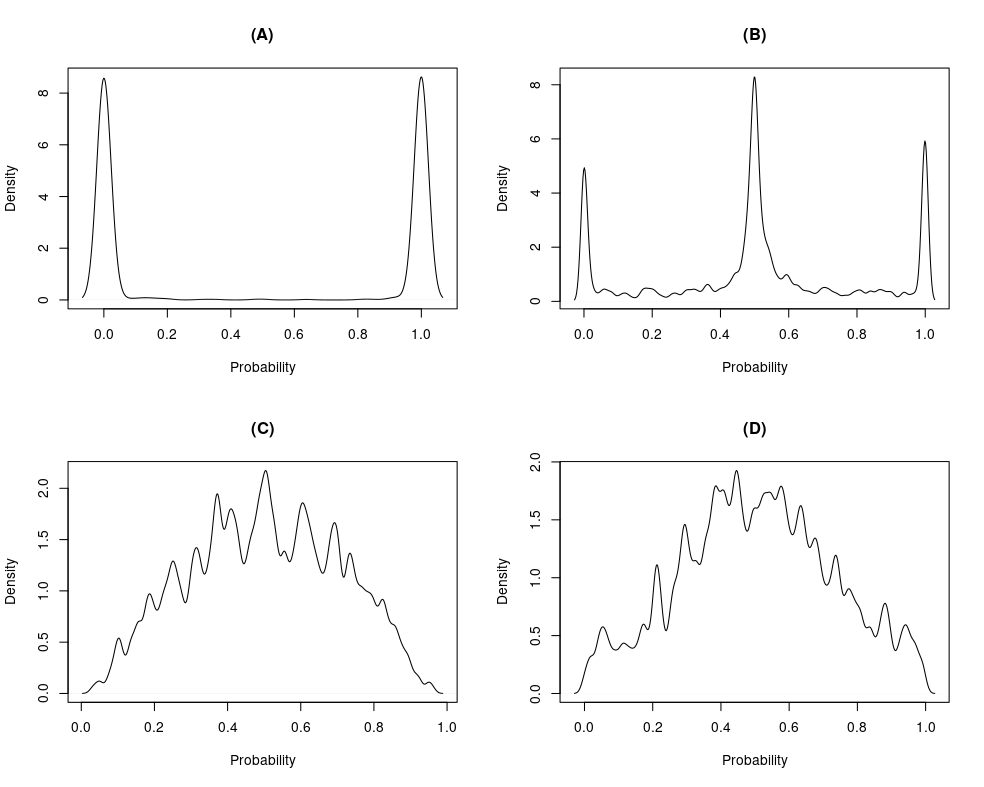
\includegraphics[width=1\textwidth]{prior_elicitation}
			\caption{Prior predictive simulation. Examples of uninformative and mildly informative priors.}
			\label{fig:prior_elicitation}
		\end{figure}
		%
	\end{frame}
	%
	%---------------------------
	\begin{frame}
		%
		\frametitle{To center or not to center}
		%
		Even the most simple hierarchical models present formidable pathologies, that no simple rotation/rescaling of the parameter can be performed to visit the posterior distribution properly \cite{Betancourt_et_al_2013}. \\
		%
		\vspace{0.3cm} Example, the devil's funnel \cite{McElreath_2020}:
		%
		%
		\begin{equation} \label{eq:devil}
			\begin{split}	
				v &\sim N(0, 3) \\
				\theta &\sim N(0, \text{exp}(v))
			\end{split}
		\end{equation}
		%
		Equation (\ref{eq:devil}) describes a centered parametrization (CP)
		%
	\end{frame}
	%
	%---------------------------
	\begin{frame}
		%
		\frametitle{To center or not to center (cont.)}
		%
		\begin{figure}[h]
			\centering
			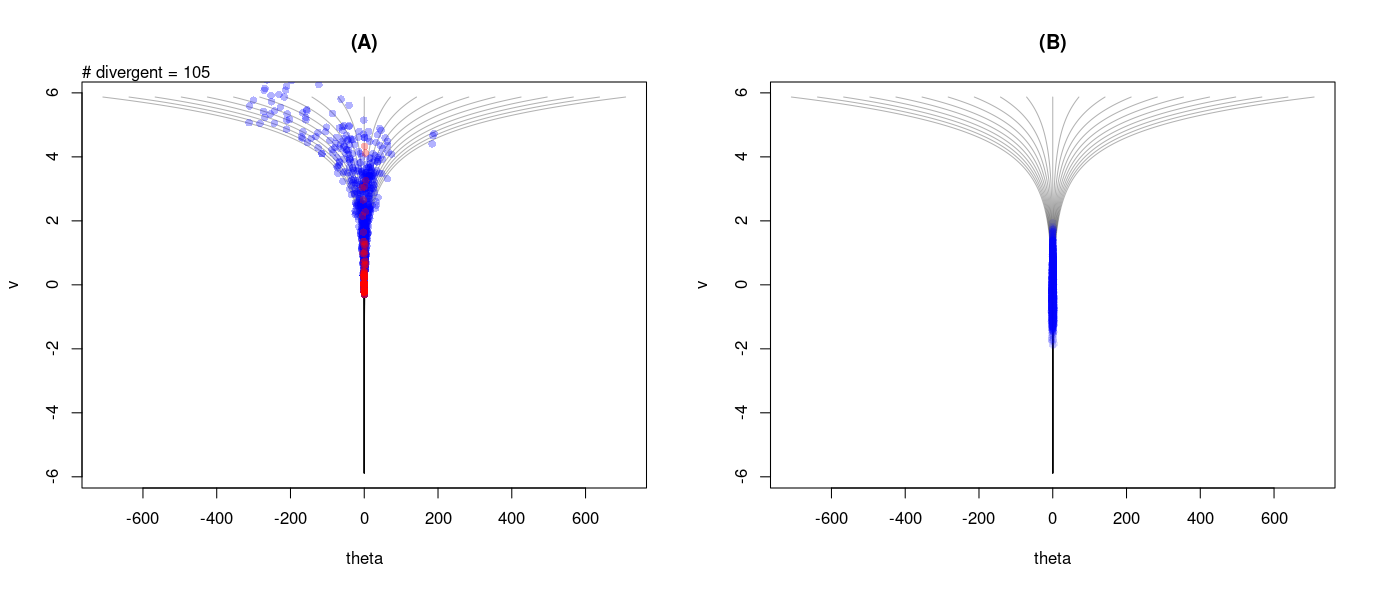
\includegraphics[width=1\linewidth]{1_funnel_CE_simple}
			%
			\caption{Posterior sampling geometry. Centered Parametrization.}
			\label{fig:devil_CE_geom}
		\end{figure}
		%
	\end{frame}
	%
	%---------------------------
	\begin{frame}
		%
		\frametitle{To center or not to center (cont.)}
		%
		\begin{figure}[h] 
			\centering
			%\begin{subfigure}
			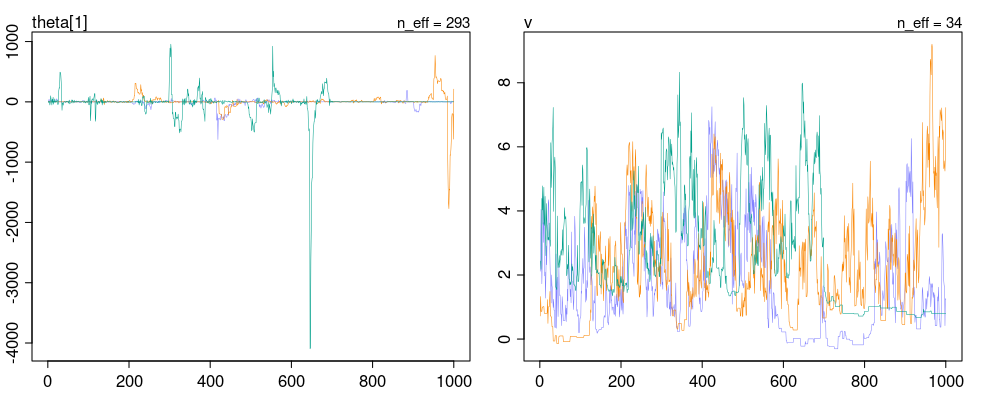
\includegraphics[width=.70\linewidth]{1_trace_CE_simple}
			%\end{subfigure}
			%
			%\begin{subfigure}
			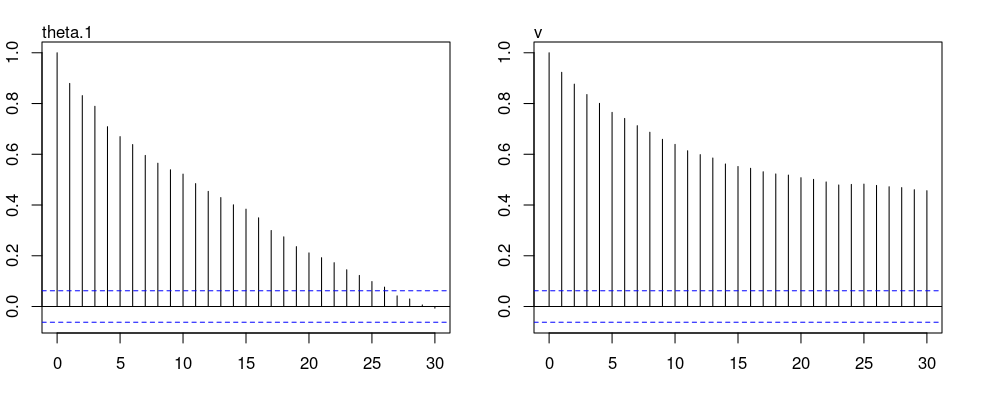
\includegraphics[width=.73\linewidth]{1_acf_CE_simple}
			%\end{subfigure}
			\caption{The Devil's funnel. Centered Parametrization. Trace and AFC plots.}
			\label{fig:devil_CE}
		\end{figure}
		%
	\end{frame}
	%
	%---------------------------
	\begin{frame}
		%
		\frametitle{To center or not to center (cont.)}
		%
		\begin{figure}[H]
			\centering
			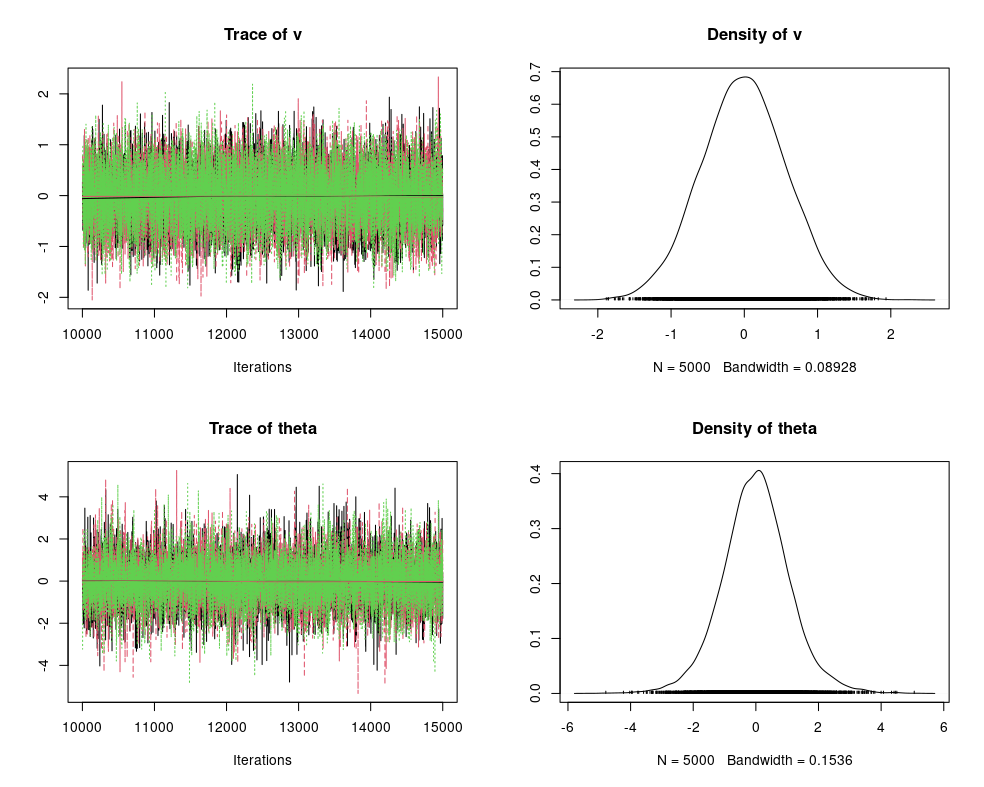
\includegraphics[width=0.7\linewidth]{1_jags_CE_simple}
			%
			\caption{The Devil's funnel. Centered Parametrization implemented in JAGS.}
			\label{fig:devil_CE_simple_jags}
		\end{figure}
		%
	\end{frame}
	%
	%---------------------------
	\begin{frame}
		%
		\frametitle{To center or not to center (cont.)}
		%
		How can we solve this?:
		%
		\begin{enumerate}
			%\setcounter{enumi}{2}
			%
			\item Adapt HMC warm-up (\texttt{adapt\_delta}$=0.99$).
			%
			\item Use \textbf{regularizing priors}
			%
			\item Use the non-centered parametrization.
			%
		\end{enumerate}
		%
	\end{frame}
	%
	%---------------------------
	\begin{frame}
		%
		\frametitle{To center or not to center \\
			(regularizing priors)}
		%
		Consider the use of a regularizing prior on equation (\ref{eq:devil}): 
		%
		\begin{equation} \label{eq:devil_prior}
			\begin{split}	
				v &\sim N(0, 1) \\
				\theta &\sim N(0, \text{exp}(v))
			\end{split}
		\end{equation}
		%
	\end{frame}
	%
	%---------------------------
	\begin{frame}
		%
		\frametitle{To center or not to center \\
			(regularizing priors, cont.)}
		%
		versus figure \ref{fig:devil_CE_geom}.
		%
		\begin{figure}[!h]
			\centering
			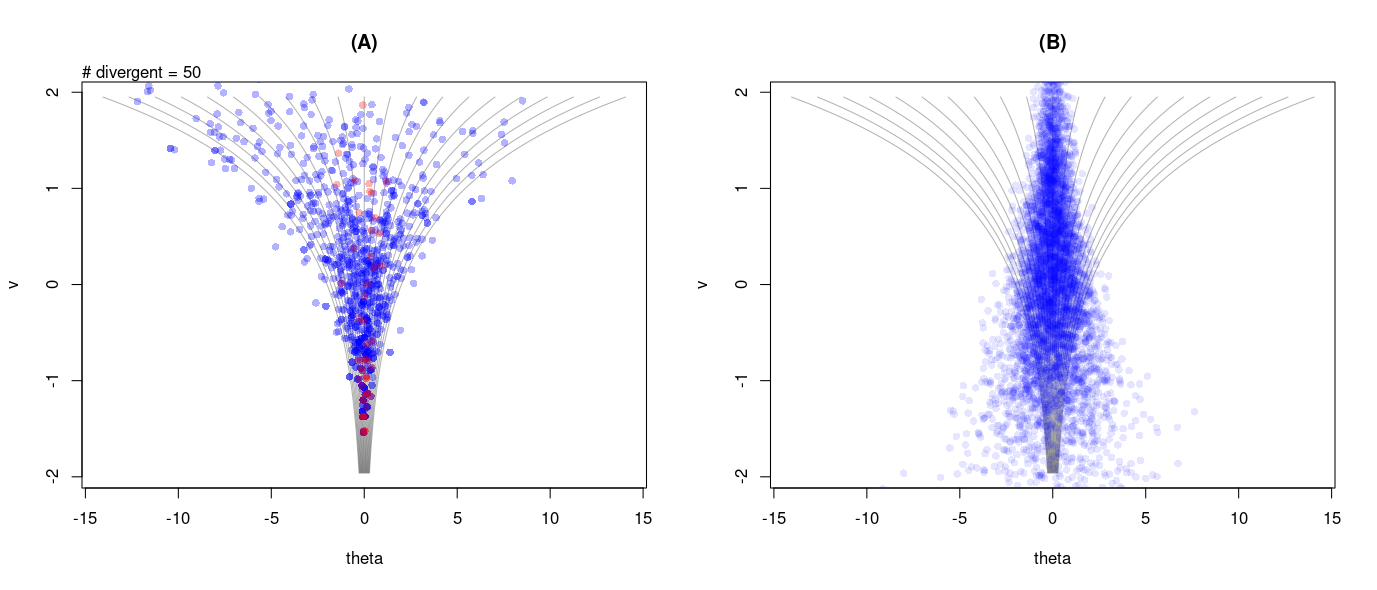
\includegraphics[width=1\linewidth]{2_funnel_CE_priors}
			\caption{Posterior sampling geometry. Centered Parametrization with mildly informative priors.}
			\label{fig:devil_prior_geom}
		\end{figure}
		%
	\end{frame}
	%
	%---------------------------
	\begin{frame}
		%
		\frametitle{To center or not to center \\
			(regularizing priors, cont.)}
		%
		versus figure \ref{fig:devil_CE}.
		%
		\begin{figure}[h] 
			\centering
			%\begin{subfigure}
			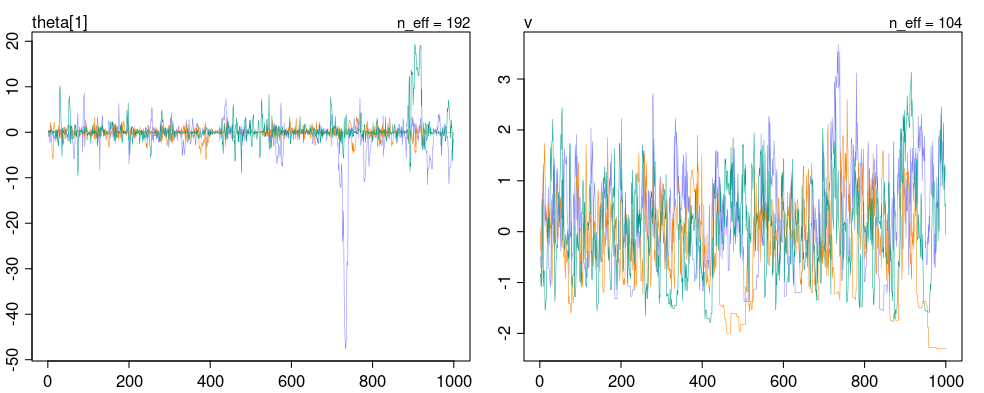
\includegraphics[width=.60\linewidth]{2_trace_CE_priors}
			%\end{subfigure}
			%
			%\begin{subfigure}
			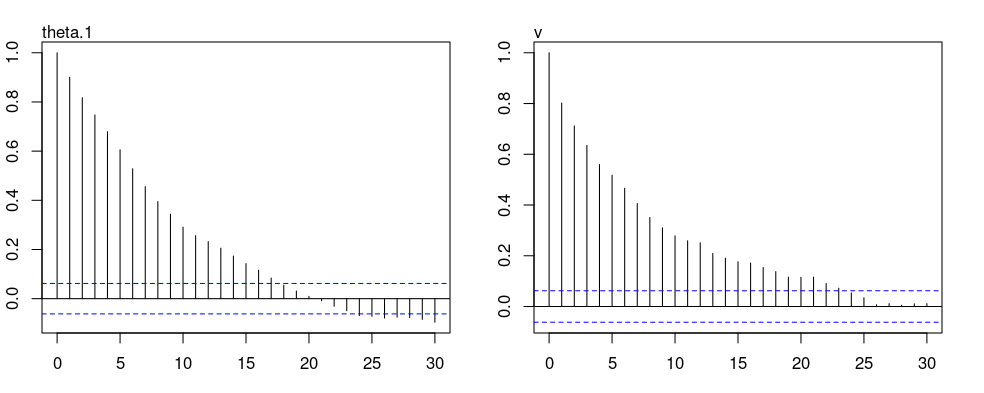
\includegraphics[width=.63\linewidth]{2_acf_CE_priors}
			%\end{subfigure}
			\caption{The Devil's funnel. Centered Parametrization with mildly informative priors. Trace and AFC plots.}
			\label{fig:devil_prior}
		\end{figure}
		%
	\end{frame}
	%
	%---------------------------
	\begin{frame}
		%
		\frametitle{To center or not to center (cont.)}
		%
		How can we solve this?:
		%
		\begin{enumerate}
			%\setcounter{enumi}{2}
			%
			\item Adapt HMC warm-up (\texttt{adapt\_delta}$=0.99$).
			%
			\item Use regularizing priors
			%
			\item Use the \textbf{non-centered parametrization}.
			%
		\end{enumerate}
		%
	\end{frame}
	%
	%---------------------------
	\begin{frame}
		%
		\frametitle{To center or not to center \\
			(non-centered parametrization)}
		%
		Changing the posterior sampling geometry means to modify equation (\ref{eq:devil}) in the following way:
		%
		\begin{equation} \label{eq:devil_NC}
			\begin{split}	
				v &\sim N(0, 3) \\
				z &\sim N(0, 1) \\
				\theta &= \text{exp}(v) \; z
			\end{split}
		\end{equation}
		%
	\end{frame}
	%
	%---------------------------
	\begin{frame}
		%
		\frametitle{To center or not to center \\
			(non-centered parametrization, cont.)}
		%
		versus figure \ref{fig:devil_CE_geom} and \ref{fig:devil_prior_geom}.
		%
		\begin{figure}[h]
			\centering
			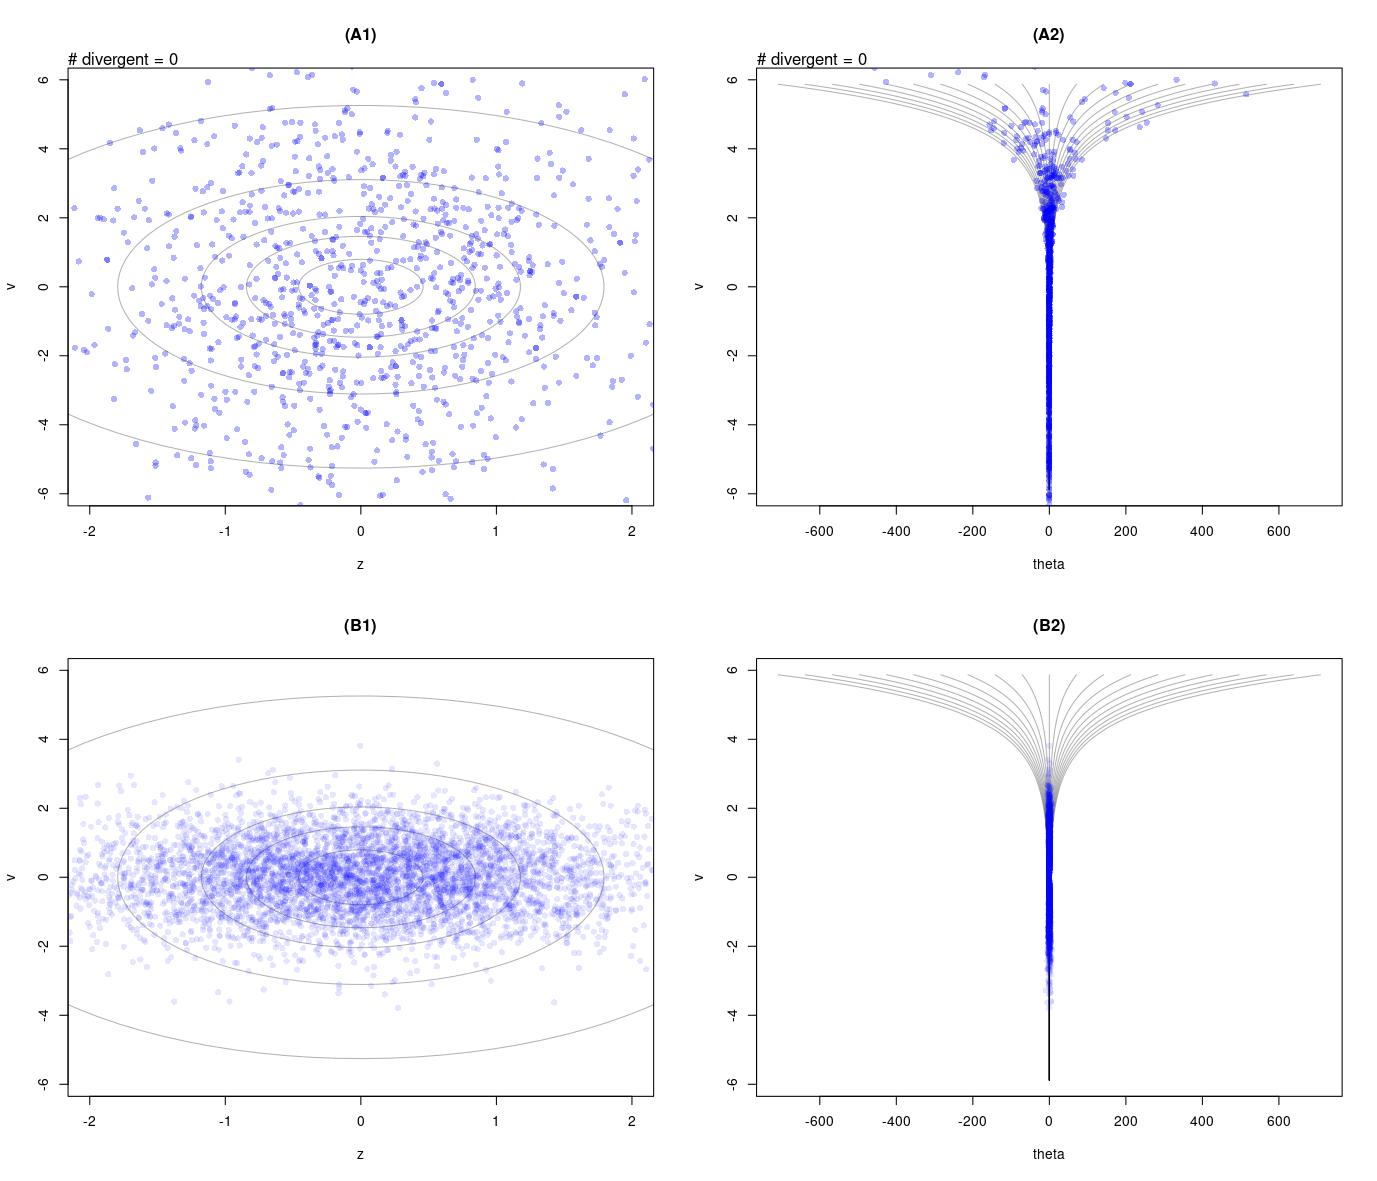
\includegraphics[width=0.60\linewidth]{3_funnel_NC}
			%
			\caption{Posterior sampling geometry. Non-Centered Parametrization.}
			\label{fig:devil_NC_geom}
		\end{figure}
		%
	\end{frame}
	%
	%---------------------------
	\begin{frame}
		%
		\frametitle{To center or not to center \\
			(non-centered parametrization, cont.)}
		%
		versus figure \ref{fig:devil_CE} and \ref{fig:devil_prior}.
		%
		\begin{figure}[h] 
			\centering
			%\begin{subfigure}
			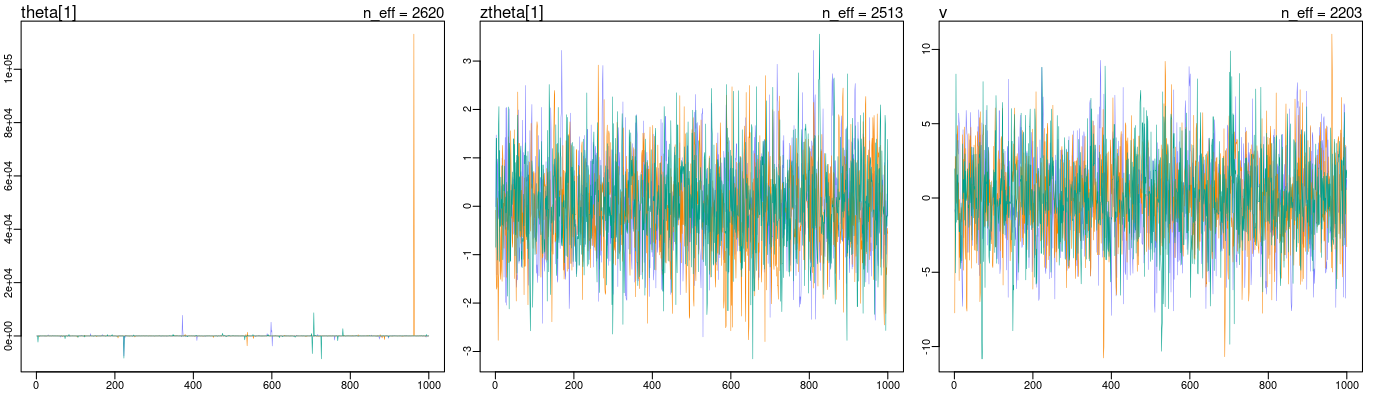
\includegraphics[width=0.85\linewidth]{3_trace_NC}
			%\end{subfigure}
			%
			%\begin{subfigure}
			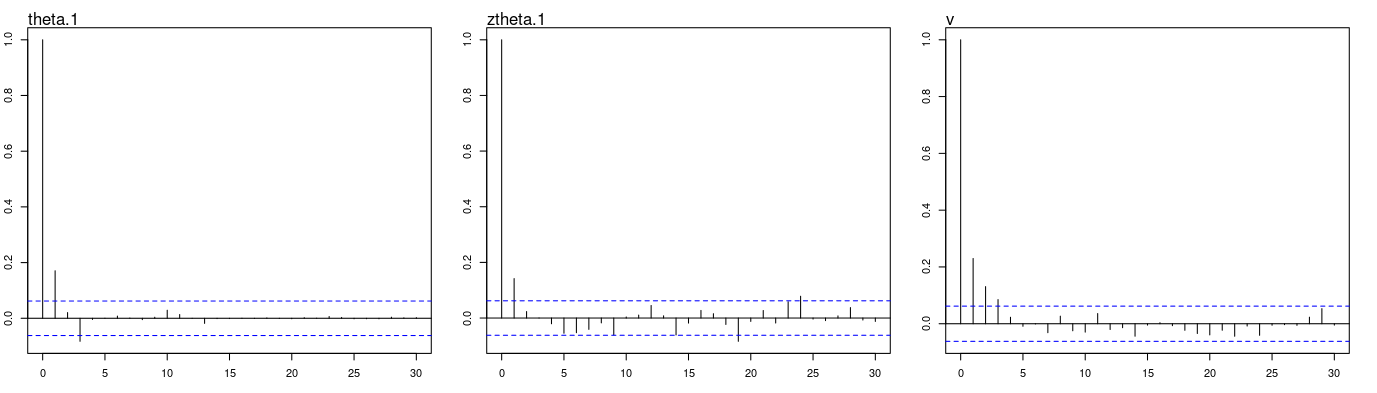
\includegraphics[width=0.88\linewidth]{3_acf_NC}
			%\end{subfigure}
			\caption{The Devil's funnel. Non-centered Parametrization. Trace and AFC plots.}
			\label{fig:devil_NC}
		\end{figure}
		%
	\end{frame}
	%
	%---------------------------
	\begin{frame}
		%
		\frametitle{Simulation \\
			(study design)}
		%
		A $3 \times 2 \times 2$ fractional factorial design:
		%
		\begin{itemize}
			\item Three different samples sizes to generate the data under analysis: $500$, $250$, and $100$.
			%
			\item Two parametrization of the models: CP and NCP.
			%
			\item Two models of interest: the first- and second-order latent variable model.
			%
		\end{itemize}
		%
		Ten ($10$) data sets were generated for each study condition. Each data set resembled responses to $25$ binary scored items, conforming to the SOLV model defined in figure \ref{fig:SOLV_model}. The model was motivated by the hypothesized structure of the reading comprehension sub-test, from the Peruvian public teaching career national assessment
		%
	\end{frame}
	%
	%---------------------------
	\begin{frame}
		%
		\frametitle{Simulation \\
			(study design, cont.)}
		%
		\begin{figure}[h]
			\centering
			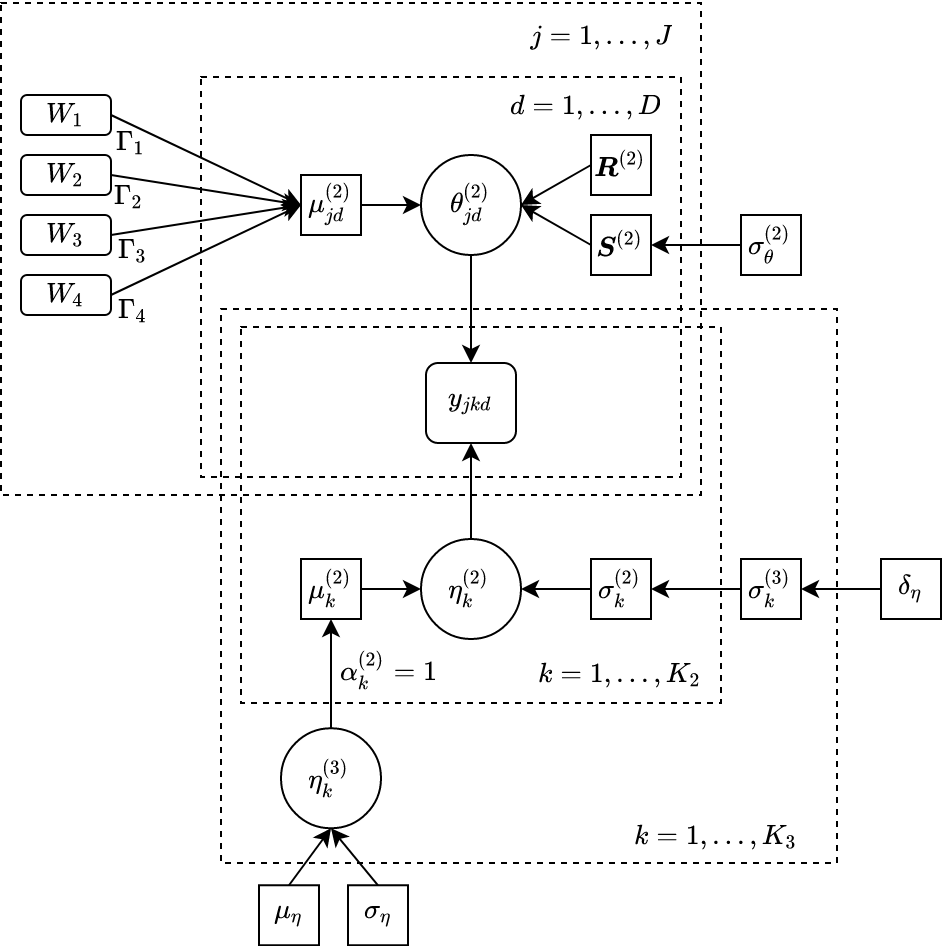
\includegraphics[width=0.60\linewidth]{4_FOLV_dag}
			%
			\caption{Directed Acyclig Graph (DAG). First-order latent variable model (SOLV).}
			\label{fig:FOLV_model}
		\end{figure}
		%
	\end{frame}
	%
	%---------------------------
	\begin{frame}
		%
		\frametitle{Simulation \\
			(study design, cont.)}
		%
		\begin{figure}[h]
			\centering
			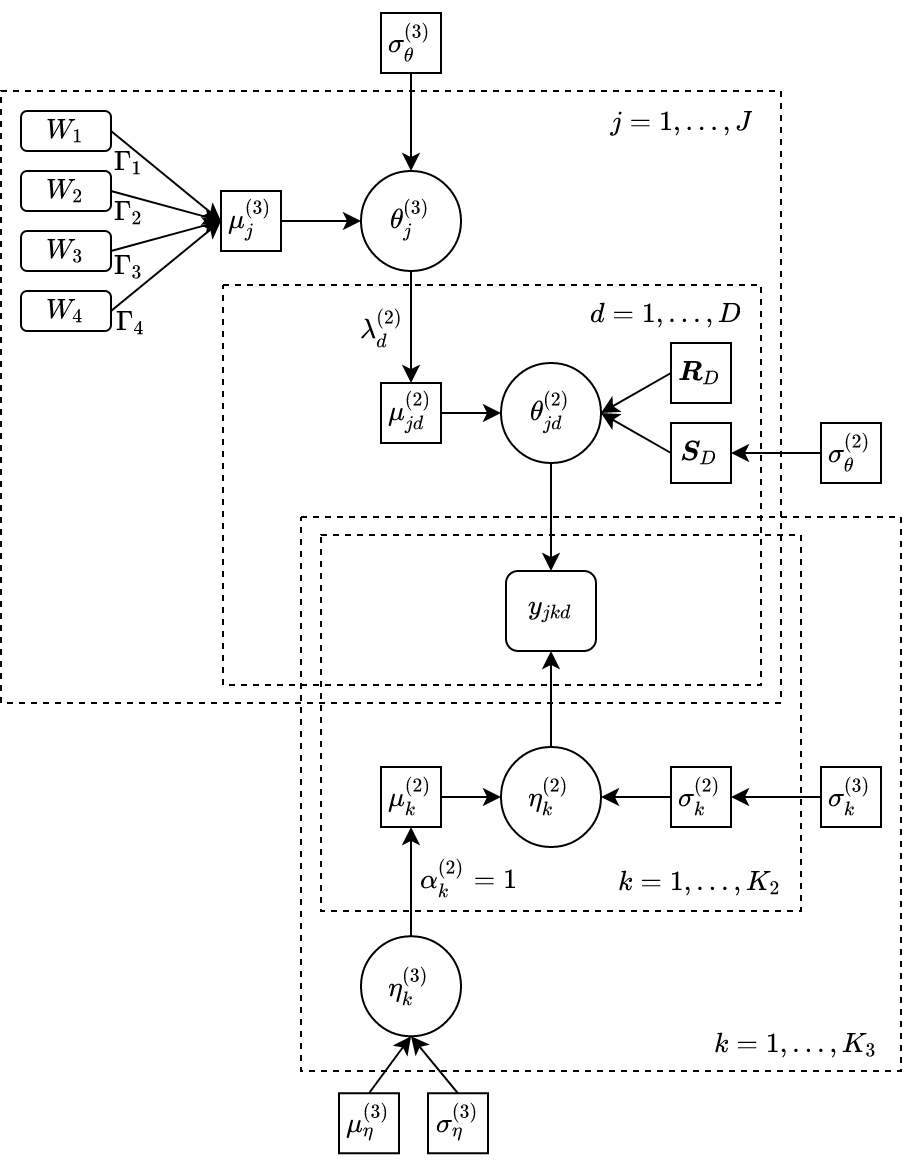
\includegraphics[width=0.57\linewidth]{4_SOLV_dag}
			%
			\caption{Directed Acyclig Graph (DAG). Second-order latent variable model (SOLV).}
			\label{fig:SOLV_model}
		\end{figure}
		%
	\end{frame}
	%
	%---------------------------
	\begin{frame}
		%
		\frametitle{Simulation \\
			(evaluation criteria)}
		%
		\begin{enumerate}
			%
			\item \textbf{Performance.} Trace, trank and ACF plots with support of \texttt{Rhat} and \texttt{n\_eff} statistics developed by \citet{Gelman_et_al_2014} (pp. $284-287$).
			%
			\item \textbf{Recovery capacity.} we used the between replica root mean squared error ($\text{RMSE}_{B}$).
			%
			\item \textbf{Retrodictive accuracy.} we used the average within $\overline{\text{RMSE}}_{W}$ and between prediction root mean squared error $\text{RMSE}_{B}$, of the responses' predictive proportion $\hat{p}$, versus the observed proportion $p$.
			%
		\end{enumerate} 
		%
	\end{frame}
	%
	%---------------------------
	\begin{frame}
		%
		\frametitle{Likelihood, priors and hyper-priors \\
			(centered parametrization)}
		%
		\begin{align}
			%
			y_{jkd} &\sim \text{Bernoulli}( \pi_{jkd} ) \\
			%
			\text{logit}( \pi_{jkd} ) &= v_{jkd} \\
			%
			v_{jkd} &= \theta^{(2)}_{jd} - \eta^{(2)}_{k}
			%
		\end{align}
		%
		\begin{align}
			%
			\boldsymbol{\theta}^{(2)}_{j} &= \left[ \theta_{j1}^{(2)}, \theta_{j2}^{(2)}, \theta_{j3}^{(2)} \right] \\
			%
			\boldsymbol{\theta}^{(2)}_{j} &\sim \text{MVNormal} \left( \boldsymbol{\mu}^{(2)}_{j}, \boldsymbol{\Sigma}^{(2)} \right) \label{eq:theta_sub}
			%
		\end{align}
		%
		%
		\begin{align} \label{eq:sigma_factoring}
			%
			\boldsymbol{\Sigma}^{(2)} &= \boldsymbol{S}^{(2)} \cdot \boldsymbol{R}^{(2)} \cdot \boldsymbol{S}^{(2)} \\
			%
			\boldsymbol{S}^{(2)} &= \pmb{\sigma}^{(2)}_{\theta} \mathbf{I}
			%
		\end{align}
		%
	\end{frame}
	%
	%---------------------------
	\begin{frame}
		%
		\frametitle{Likelihood, priors and hyper-priors \\
			(centered parametrization, cont.)}
		%
		For the FOLV model:
		%
		\begin{align}
			%
			\boldsymbol{\mu}^{(2)}_{j} &= \left[ \mu^{(2)}_{j1}, \; \mu^{(2)}_{j2}, \mu^{(2)}_{j3} \right] \label{eq:mu_FOLV} \\
			%
			\mu^{(2)}_{jd} &= \Gamma_{0} + \Gamma_{1} W_{1j} + \Gamma_{2} (W_{2j} - W_{2\text{min}}) + \Gamma_{3} W_{3j} + \Gamma_{4} W_{4j}
			%
		\end{align}
		%
	\end{frame}
	%
	%---------------------------
	\begin{frame}
		%
		\frametitle{Likelihood, priors and hyper-priors \\
			(centered parametrization, cont.)}
		%
		For the SOLV model:
		%
		\begin{align}
			%
			\boldsymbol{\mu}^{(2)}_{j} &= \left[ \mu^{(2)}_{j1}, \; \mu^{(2)}_{j2}, \mu^{(2)}_{j3} \right] \\
			%
			\pmb{\lambda}^{(2)} &= \left[ \lambda^{(2)}_{1}, \; \lambda^{(2)}_{2}, \lambda^{(2)}_{3} \right] \\
			%
			\mu^{(2)}_{jd} &= \lambda^{(2)}_{d} \; \theta^{(3)}_{j} 
			%
		\end{align}
		%
		%
		\begin{align}
			%
			\theta^{(3)}_{j} &\sim \text{Normal} \left( \mu^{(3)}_{j}, \sigma^{(3)}_{\theta} \right) \label{eq:theta} \\
			%
			\mu^{(3)}_{j} &=  \Gamma_{0} + \Gamma_{1} W_{1j} + \Gamma_{2} (W_{2j} - W_{2\text{min}}) + \Gamma_{3} W_{3j} + \Gamma_{4} W_{4j} \label{eq:mu_SOLV}
		\end{align}
		%
	\end{frame}
	%
	%---------------------------
	\begin{frame}
		%
		\frametitle{Likelihood, priors and hyper-priors \\
			(centered parametrization, cont.)}
		%
		For the items:
		%
		\begin{align}
			%
			\eta^{(2)}_{k} &\sim \text{Normal} \left( \mu^{(2)}_{k}, \sigma^{(2)}_{k} \right) \label{eq:items} \\
			%
			\mu^{(2)}_{k} &= \pmb{\eta}^{(3)} \mathbf{A} \label{eq:mu_items} \\
			%
			\sigma^{(2)}_{k} &= \pmb{\sigma}^{(3)} \mathbf{A} \label{eq:sigma_items} \\
			%
			\pmb{\eta}^{(3)} &= [ \eta^{(3)}_{1}, \eta^{(3)}_{2}, \eta^{(3)}_{3}, \eta^{(3)}_{4}, \eta^{(3)}_{5} ] \\
			%
			\pmb{\sigma}^{(3)} &= [ \sigma^{(3)}_{1}, \sigma^{(3)}_{2}, \sigma^{(3)}_{3}, \sigma^{(3)}_{4}, \sigma^{(3)}_{5} ]
			%
		\end{align}
		%
		\begin{align}
			%
			\eta^{(3)}_{k} &\sim \text{Normal} \left( \mu_{\eta}, \sigma_{\eta} \right) \\
			%
			\sigma^{(3)}_{k} &\sim \text{Exponential} \left( \delta_{\eta} \right)
			%
		\end{align}
		%
	\end{frame}
	%
	%---------------------------
	\begin{frame}
		%
		\frametitle{Likelihood, priors and hyper-priors \\
			(centered parametrization, cont.)}
		%
		Remaining priors and hyper-priors
		%
		\begin{align}
			\boldsymbol{R}^{(2)} &\sim \text{LkjCorrelation}( 2 ) \\
			\Gamma_{1c} &\sim \text{Normal}( 0, 0.5 ) \\
			\Gamma_{2} &\sim \text{Normal}( 0, 0.5 ) \\
			\Gamma_{3c} &\sim \text{Normal}( 0, 1 ) \\
			\Gamma_{4c} &\sim \text{Normal}( 0, 0.5 ) 
			%
		\end{align}
		%
	\end{frame}
	%
	%---------------------------
	\begin{frame}
		%
		\frametitle{Likelihood, priors and hyper-priors \\
			(Non-centered parametrization)}
		%
		Under the NCP, equation (\ref{eq:items}) was re-defined as follows:
		%
		\begin{align}
			%
			\eta^{(2)}_{k} &= \mu^{(2)}_{k} + \sigma^{(2)}_{k} z^{(2)}_{k} \\
			%
			z^{(2)}_{k} &\sim \text{Normal}(0,1)
			%
		\end{align}
		%
		Equation (\ref{eq:theta_sub}) was re-defined as follows:
		%
		\begin{align}
			%
			\boldsymbol{\theta}^{(2)}_{j} &= \boldsymbol{\mu}^{(2)}_{j} + \boldsymbol{S}^{(2)} \cdot \boldsymbol{L}^{(2)}_{\Sigma} \cdot  (\mathbf{z}_{j} \mathbf{I}) \\
			%
			\mathbf{z}_{j} &= [ z_{j1}, \dots, z_{jd}]^{T} \\
			%
			z_{jd} &\sim \text{Normal}(0,1) \\
			%
			\boldsymbol{L}^{(2)}_{\Sigma} &\sim \text{LKJCorrelationCholesky}(2)
			%
		\end{align}
		%
	\end{frame}
	%
	%---------------------------
	\begin{frame}
		%
		\frametitle{Likelihood, priors and hyper-priors \\
			(Non-centered parametrization, cont.)}
		%
		Finally, equation (\ref{eq:theta}) was re-defined as follows:
		%
		\begin{align}
			%
			\theta^{(3)}_{j} &= \mu^{(3)}_{j} + \sigma^{(3)}_{\theta} z_{j} \\
			%
			z_{j} &\sim \text{Normal}(0,1)
			%
		\end{align}
		%
	\end{frame}
	%
	%---------------------------
	\begin{frame}
		%
		\frametitle{Identification}
		%
		We used the unit variance identification scheme (UVI), that is, to set the scale of the higher-order dimension and sub-dimensions to one:
		%
		\begin{itemize}
			\item $\sigma^{(3)}_{\theta} = 1$
			%
			\item $\mathbf{S}^{(2)} = \pmb{\sigma}^{(2)}_{\theta} \mathbf{I}$ with $\pmb{\sigma}^{(2)}_{\theta} = [1, 1, 1]^{T}$
			%
			\item $\mu_{\eta} = 0$, $\sigma_{\eta}=1$, $\delta_{\eta}=2$
		\end{itemize}
		%
		The second turned the covariance matrix into a correlation, i.e. $\boldsymbol{\Sigma}^{(2)} = \boldsymbol{R}^{(2)}$.
		%
	\end{frame}
	%
	%---------------------------
	\begin{frame}
		%
		\frametitle{Prior predictive investigation}
		%
		From two perspectives:
		%
		\begin{itemize}
			\item the IRT perspective
			%
			\item the outcome perspective
		\end{itemize}
		% 
	\end{frame}
	%
	%---------------------------
	\begin{frame}
		%
		\frametitle{Prior predictive investigation (cont.)}
		%
		From the IRT perspective:
		%
		\begin{figure}[H]
			\centering
			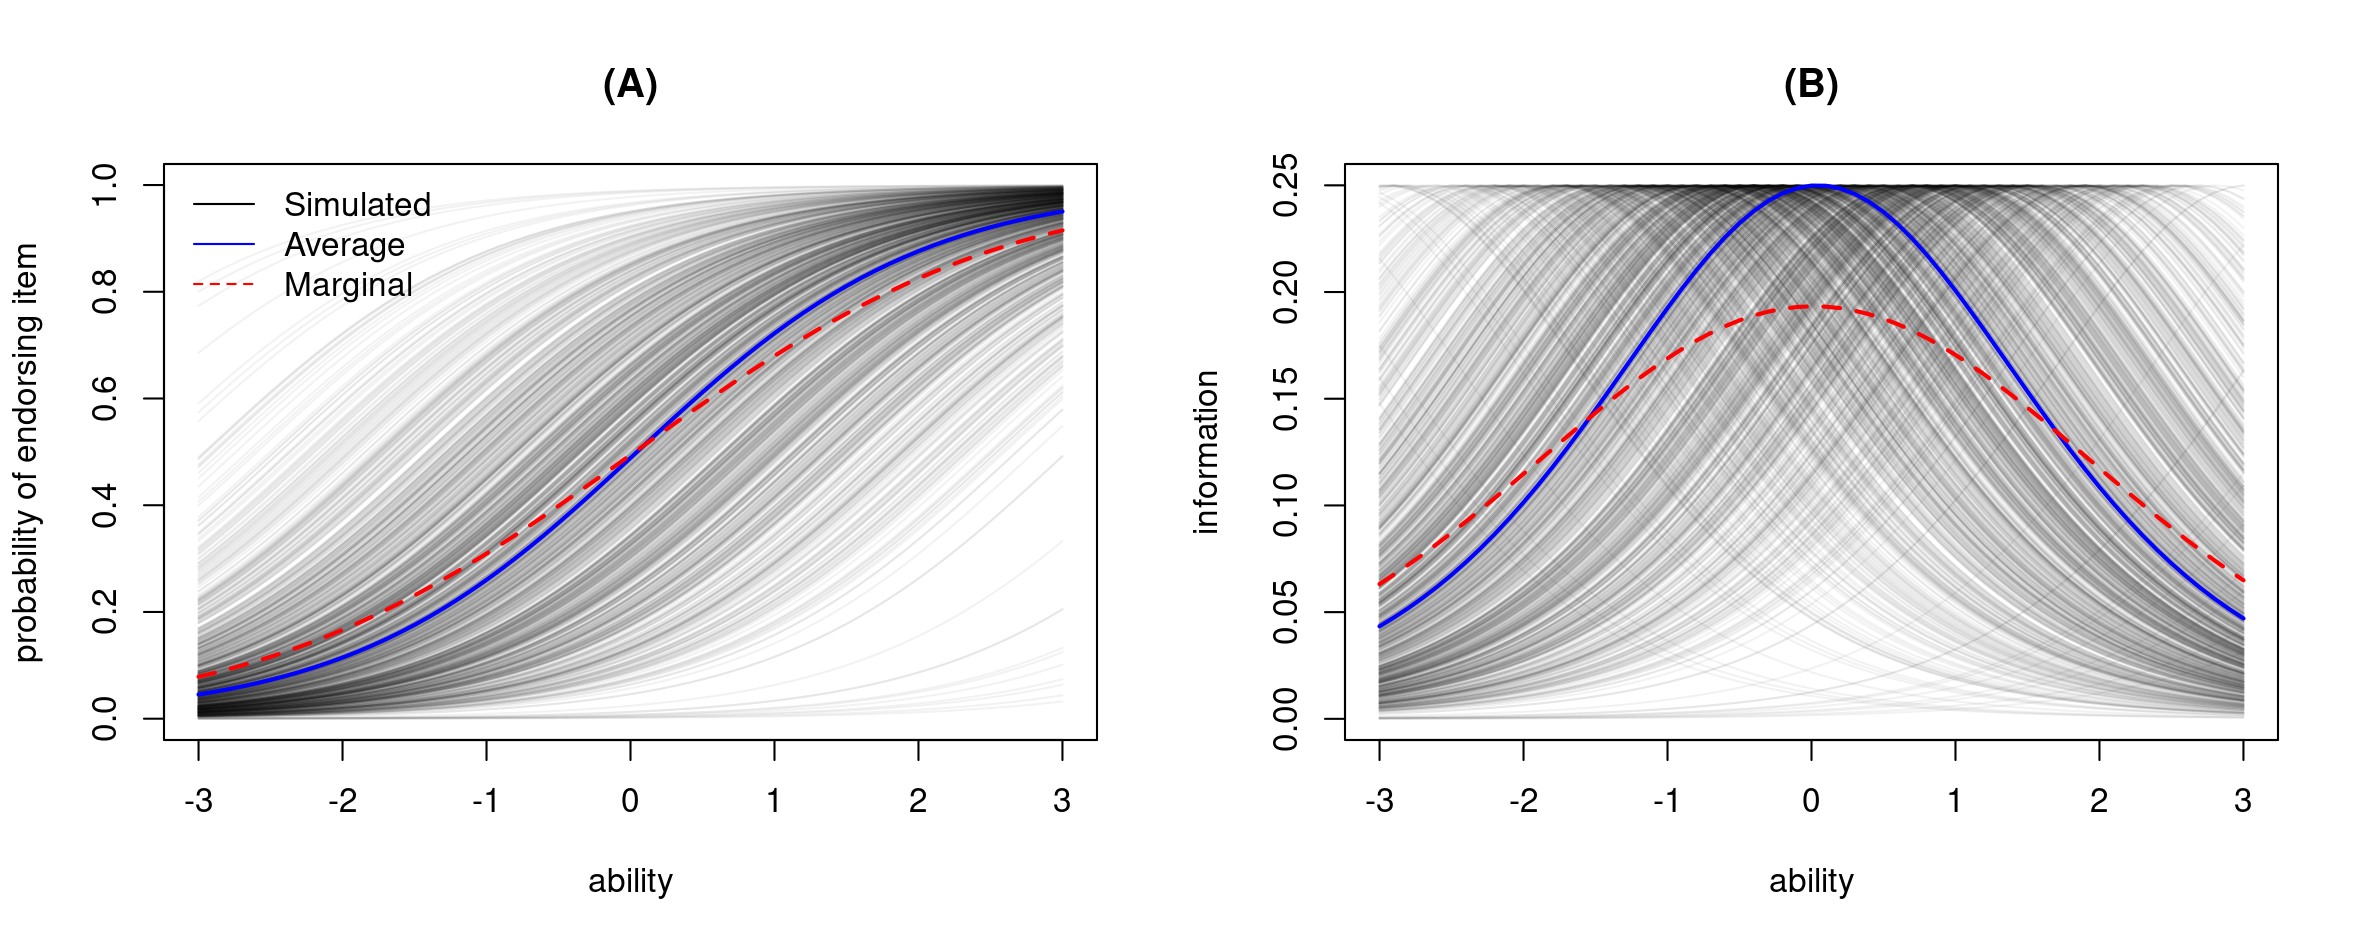
\includegraphics[width=1\linewidth]{FOLV_ICC_prior}
			%
			\caption{First-order latent variable model (FOLV). (A) Item Characteristics Curve, ICC. (B) Item Information Function, IIF.}
			\label{fig:FOLV_ICC_prior}
		\end{figure} 
		%
	\end{frame}
	%
	%---------------------------
	\begin{frame}
		%
		\frametitle{Prior predictive investigation (cont.)}
		%
		From the outcome perspective:
		%
		\begin{figure}[h]
			\centering
			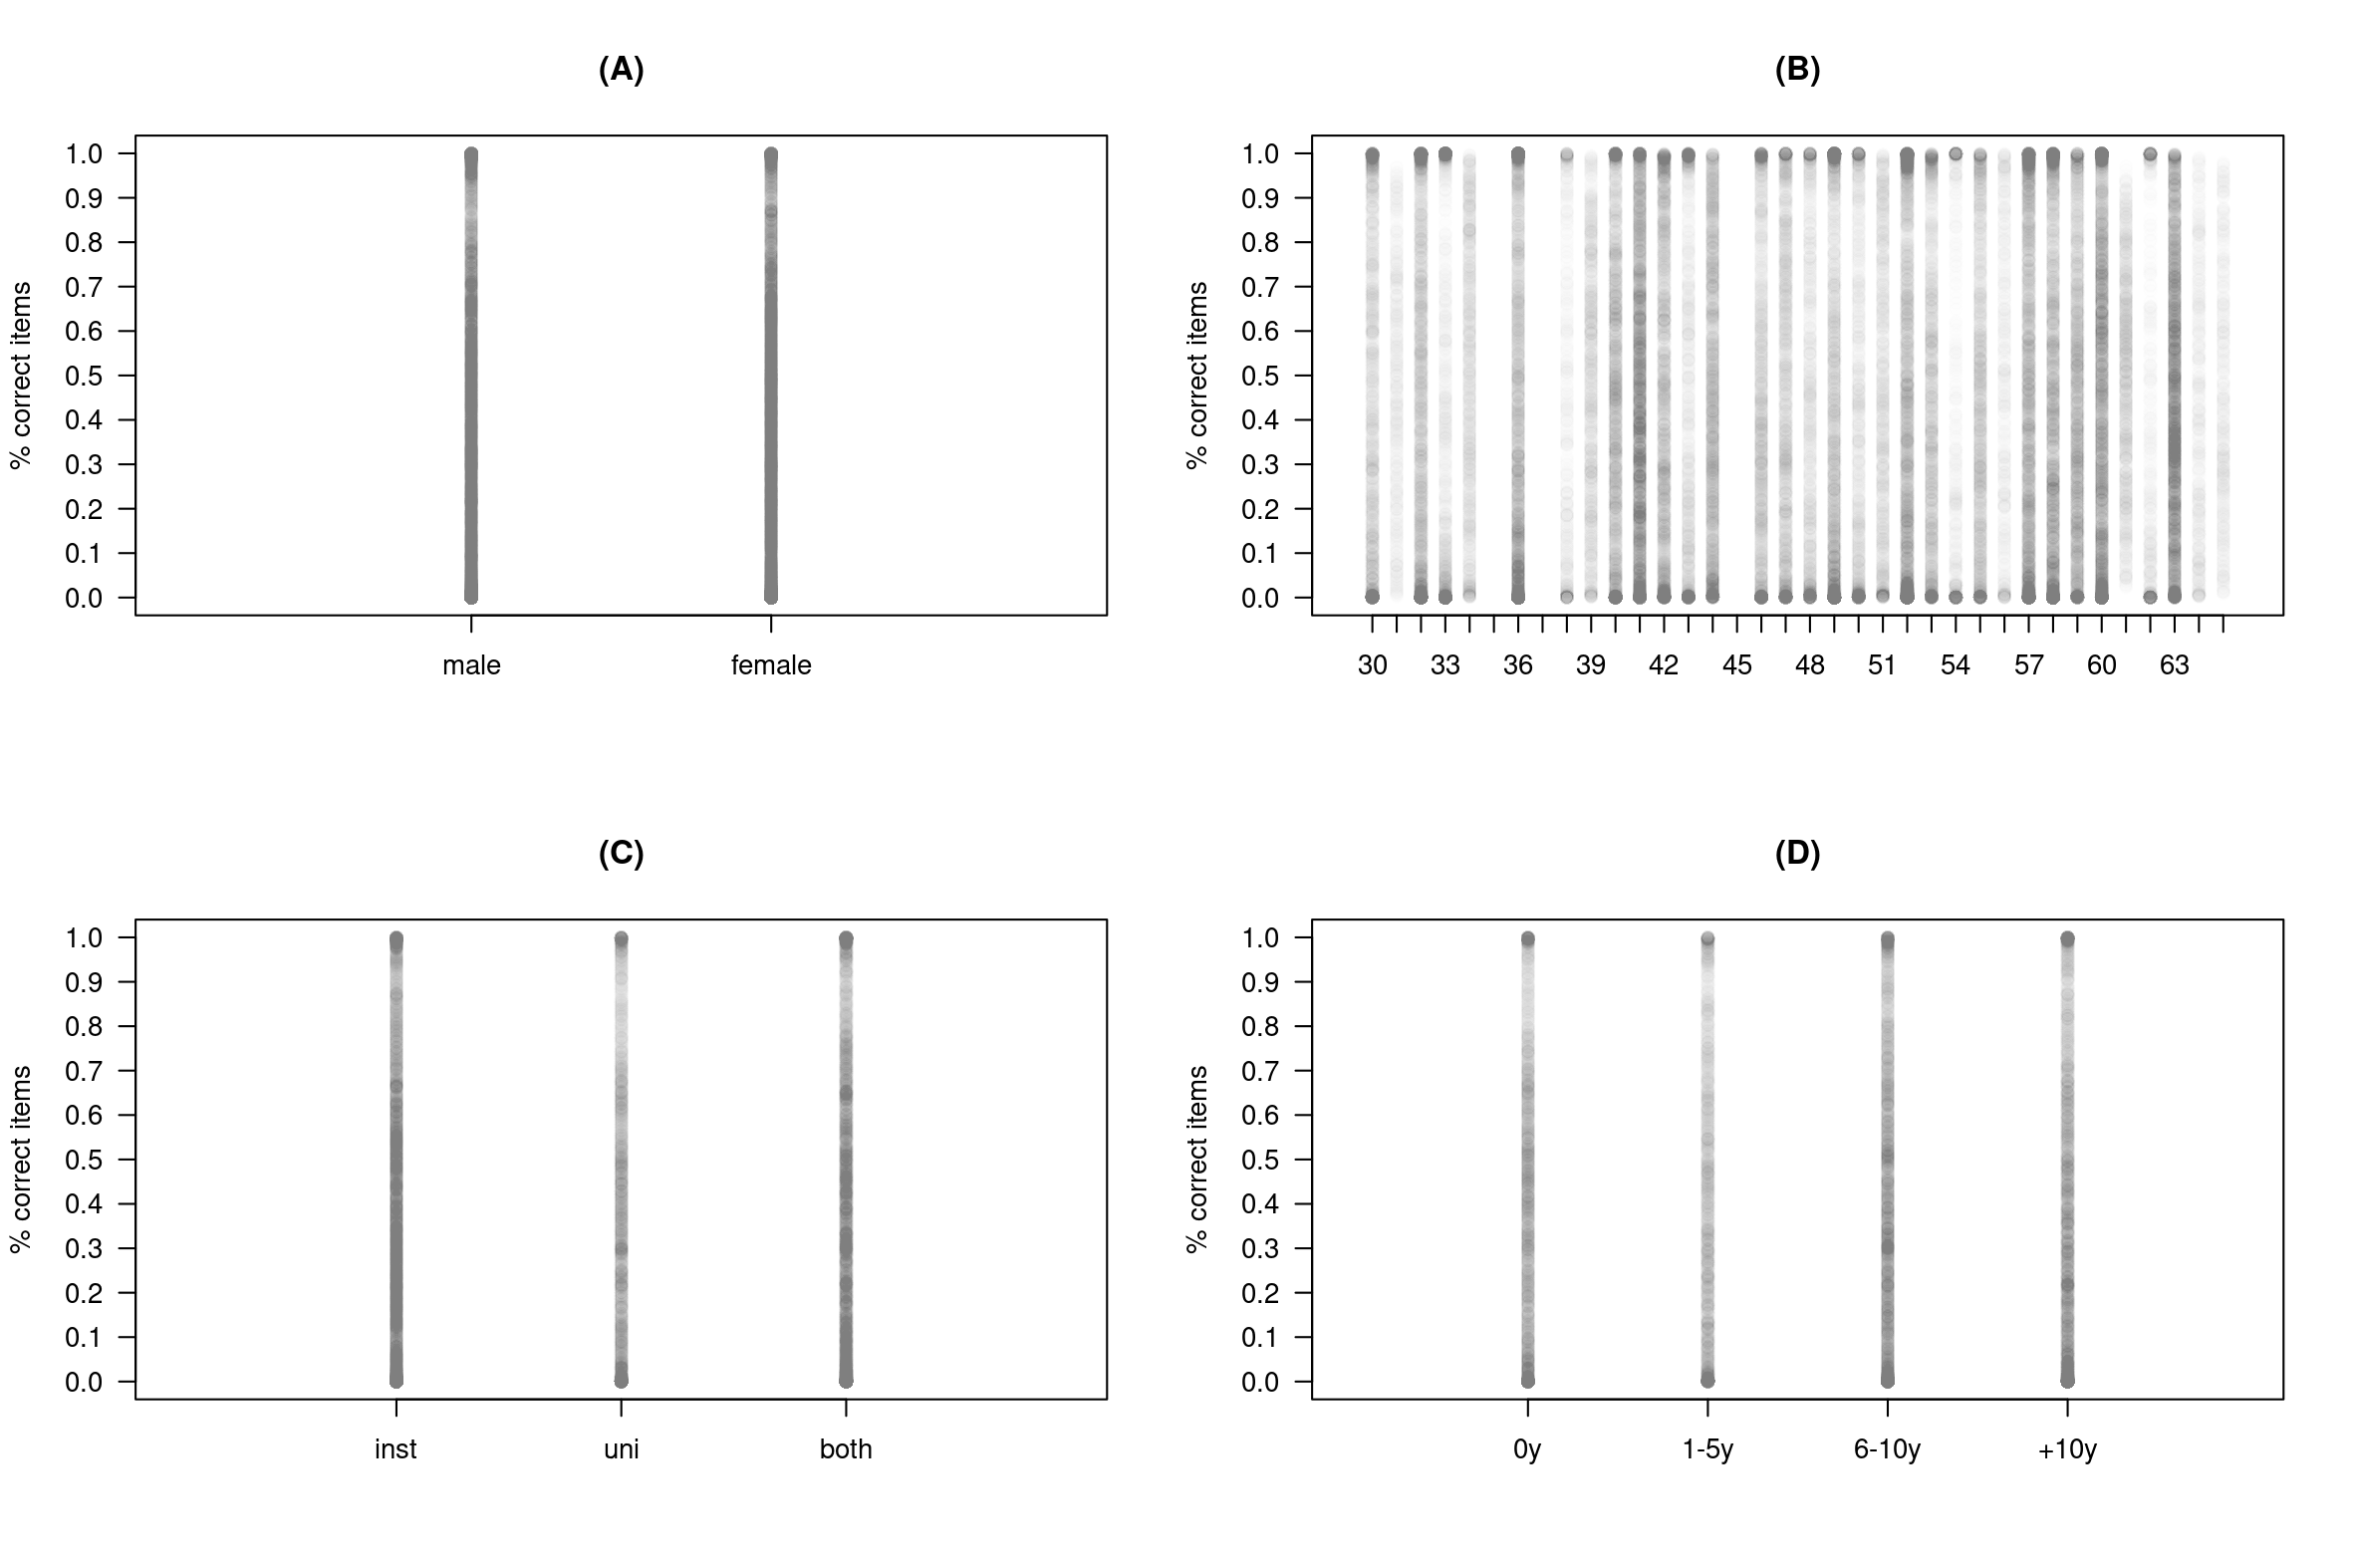
\includegraphics[width=0.65\linewidth]{FOLV_HitRate2}
			%
			\caption{First-order latent variable model (FOLV). Aggregated endorsement rate per simulated covariate: (A) gender, (B) age, (C) education, and (D) experience.}
			\label{fig:FOLV_hitrate2}
		\end{figure}
		% 
	\end{frame}
	%
	%---------------------------
	\begin{frame}
		%
		\frametitle{Running time }
		%
		\begin{table}[h]
			\centering
			\begin{tabular}{rlrrrr}
				\hline
				\multicolumn{3}{c}{ }& \multicolumn{3}{c}{ Time (min.) } \\ 
				\cmidrule(rl){4-6} 
				& Parametrization & Sample & mean & min & max \\ 
				\hline\hline
				1 & CP & 100 & 4.80 & 1.89 & 7.56 \\ 
				2 & CP & 250 & 7.85 & 5.60 & 16.57 \\ 
				3 & CP & 500 & 19.15 & 17.20 & 22.53 \\ 
				%
				\hline
				%
				4 & NCP & 100 & 1.94 & 1.74 & 2.23 \\ 
				5 & NCP & 250 & 7.18 & 6.78 & 8.40 \\ 
				6 & NCP & 500 & 22.38 & 20.12 & 28.62 \\
				\hline
			\end{tabular}
			\caption{First-order latent variable model (FOLV). Running time statistics.} 
			\label{tab:FOLV_time}
		\end{table}
		% 
	\end{frame}
	%
	%---------------------------
	\begin{frame}
		%
		\frametitle{Running time (cont.)}
		%
		\begin{table}[h]
			\centering
			\begin{tabular}{rlrrrr}
				\hline
				\multicolumn{3}{c}{ }& \multicolumn{3}{c}{ Time (min.) } \\ 
				\cmidrule(rl){4-6} 
				& Parametrization & Sample & mean & min & max \\ 
				\hline\hline
				1 & CP & 100 & 4.04 & 1.39 & 8.55 \\ 
				2 & CP & 250 & 7.13 & 5.22 & 11.49 \\ 
				3 & CP & 500 & 16.14 & 14.45 & 19.73 \\ 
				%
				\hline
				%
				4 & NCP & 100 & 1.87 & 1.62 & 2.28 \\ 
				5 & NCP & 250 & 5.92 & 5.20 & 6.79 \\ 
				6 & NCP & 500 & 16.58 & 13.37 & 18.26 \\
				\hline
			\end{tabular}
			\caption{Second-order latent variable model (SOLV). Running time statistics.} 
			\label{tab:SOLV_time}
		\end{table}
		% 
	\end{frame}
	%
	%---------------------------
	\begin{frame}
		%
		\frametitle{Application \\
			(model fit)}
		%
		They try to approximate the out-of-sample KL-divergence \cite{Kullback_et_al_1951}:
		%
		\begin{table}[H]
			\centering
			\begin{tabular}{rlrrrr}
				\hline
				& Model & Param. & WAIC & lppd & penalty \\  
				\hline\hline
				1 & FOLV & CP &  54,632.4 & -25,429.7 & 1,886.5 \\ 
				2 & FOLV & NCP & 54,631.7 & -25,427.6 & 1,888.3 \\
				%
				\hline
				%
				3 & SOLV & CP &  54,610.3 & -25,348.4 & 1,956.7 \\  
				4 & SOLV & NCP & 54,614.7 & -25,337.9 & 1,969.4 \\ 
				\hline
			\end{tabular}
			\caption[Model fit. Widely Applicable Information Criterion (WAIC).]%
			{Model fit. Widely Applicable Information Criterion (WAIC).}
			\label{tab:model_fit1}
		\end{table}
		% 
	\end{frame}
	%
	%---------------------------
	\begin{frame}
		%
		\frametitle{Application \\
			(model fit, cont.)}
		%
		\begin{table}[H]
			\centering
			\begin{tabular}{rlrrrr}
				\hline
				& Model & Param. & PSIS & lppd & penalty \\  
				\hline\hline
				1 & FOLV & CP &  54,657.4 & -27,328.7 & 1,904.4 \\ 
				2 & FOLV & NCP & 54,656.9 & -27,328.5 & 1,898.1  \\
				%
				\hline
				%
				3 & SOLV & CP &  54,627.3 & -27,313.7 & 1,940.1 \\  
				4 & SOLV & NCP & 54,642.5 & -27,321.2 & 1,990.2 \\ 
				\hline
			\end{tabular}
			\caption[Model fit. Pareto-smoothed importance sampling cross-validation (PSIS).]%
			{Model fit. Pareto-smoothed importance sampling cross-validation (PSIS).}
			\label{tab:model_fit2}
		\end{table} 
		% 
	\end{frame}
	%
	%
	%%%%%%%%%%%%%%%%%%%%%%%%%%%%%%%%%%%%%%%%%%%%%%%%%%%%%%%%%%%%%%%%%
	% Bibliography
	%%%%%%%%%%%%%%%%%%%%%%%%%%%%%%%%%%%%%%%%%%%%%%%%%%%%%%%%%%%%%%%%%
	%
	\begin{frame}[allowframebreaks]
		\frametitle{References}
		%
		%\renewcommand{\harvardand}{y} 	% cambiar "and" por "y" al generar la bibliografia.
		\bibliographystyle{dcu}
		\bibliography{bibliography}
		%
	\end{frame}
	%
	%
\end{document}
